\documentclass[12pt]{article}
\usepackage{graphicx} % Required for inserting images
\usepackage[utf8]{vietnam}
\usepackage[]{amsthm} %lets us use \begin{proof}
\usepackage[]{amssymb} %gives us the character \varnothing
\usepackage[section]{placeins}
\usepackage{fancybox}
\usepackage{indentfirst}
\usepackage{float}
\usepackage{geometry}
\usepackage{subcaption} % For subfigure environment
\usepackage{hyperref}
\usepackage{listings}
\usepackage{fancyhdr}
\usepackage{color}
\usepackage{extsizes}
\usepackage{tcolorbox}
\usepackage{setspace}
\usepackage{caption}
\usepackage{xcolor}
\usepackage{amsmath}
\usepackage{tabularx}
\usepackage{ragged2e}
\usepackage{enumitem}
\usepackage{bm}
\usepackage{comment}
\usepackage{booktabs}
\usepackage{xltabular}
\usepackage{tikz}
\usetikzlibrary{shapes,arrows.meta,positioning,fit,backgrounds,calc}

\hypersetup{
    colorlinks=true,
    linkcolor=black,
    citecolor=black,
    urlcolor=blue,
}

\renewcommand{\normalsize}{\fontsize{13}{15}\selectfont}
\geometry{left = 2cm, right = 2cm}
\lstset{
    basicstyle=\ttfamily\footnotesize,
    keywordstyle=\color{blue},
    commentstyle=\color{green!50!black},
    stringstyle=\color{red},
    numbers=left,
    numberstyle=\tiny\color{gray},
    stepnumber=1,
    frame=single,
    breaklines=true,
    captionpos=b,
    tabsize=2
}

\setstretch{1.2}
% Cho phép giãn khoảng trắng ở dòng có tên file/lệnh (\texttt) dài, tránh chữ tràn lề
\setlength{\emergencystretch}{3em}

\begin{document}
\justifying
\newgeometry{left=2cm,right=2cm,top=2cm,bottom=2cm}
\thispagestyle{empty}

\begin{center}
    \textbf{\Large ĐẠI HỌC QUỐC GIA THÀNH PHỐ HỒ CHÍ MINH}\\
    \textbf{\Large TRƯỜNG ĐẠI HỌC BÁCH KHOA}\\
    \textbf{\large KHOA KHOA HỌC VÀ KỸ THUẬT MÁY TÍNH}\\[1cm]

    % Logo BK
    
\includegraphics[width=0.35\textwidth]{logoBK.png}\\[1cm]

    \textbf{\Large BÁO CÁO BÀI TẬP LỚN}\\[0.2cm]
    \textbf{\Large KHO DỮ LIỆU VÀ HỆ HỖ TRỢ QUYẾT ĐỊNH}\\[0.4cm]
    \rule{0.8\textwidth}{0.4pt}\\[0.6cm]

    \textbf{\Huge XÂY DỰNG KHO DỮ LIỆU VÀ}\\[0.2cm]
    \textbf{\Huge HỆ HỖ TRỢ QUYẾT ĐỊNH CHO}\\[0.2cm]
    \textbf{\Huge THƯƠNG MẠI ĐIỆN TỬ}\\[0.6cm]

    \rule{0.8\textwidth}{0.4pt}
\end{center}

\vspace{1cm}

\begin{flushleft}
\hspace{2cm}
\begin{tabular}{l l}
    \textbf{Giảng viên hướng dẫn:} & TS. Đỗ Thanh Thái \\
    % \textbf{Nhóm:} & Nhóm \_\_\_ \\
    \textbf{Sinh viên:} & Phan Ngọc Quỳnh Trang - 2313518 \\
    \textbf{} & Nguyễn Thanh Hùng - 2411324 \\
    \textbf{} & Quách Văn Hà - 2410858 \\
\end{tabular}
\end{flushleft}

\vfill
% \vspace{0.3cm}

\begin{center}
    {\footnotesize TP. HỒ CHÍ MINH, THÁNG 11/2026}
\end{center}

\thispagestyle{empty}
\newpage
\tableofcontents
\thispagestyle{empty}
\clearpage
\fancyhf{}
\pagestyle{fancy}
\fancyhead{}

\renewcommand{\footruleskip}{1mm}

\fancyhead[L]{
 \begin{tabular}{rl}
    \begin{picture}(25,15)(0,0)
    \put(0,-8){
\includegraphics[width=15mm, height=15mm]{logoBK.png}}
   \end{picture}&
	\begin{tabular}{l}
		\textbf{  Trường Đại Học Bách Khoa - Đại học Quốc gia TP.HCM }\\
		\textbf{  Khoa Khoa Học \& Kỹ Thuật Máy Tính}
	\end{tabular}
 \end{tabular}
}
\fancyhead[R]{
	\begin{tabular}{l}
		\tiny \bf \\
		\tiny \bf
	\end{tabular}
}
\fancyfoot[R]{\thepage}
\fancyfoot[L]{\textbf{Kho dữ liệu \& Hệ hỗ trợ Quyết định (CO4031)}}
\renewcommand{\footrulewidth}{1pt}
\setlength{\headheight}{32pt}
\setlength{\headsep}{1.5cm}
\setlength{\footskip}{1cm}

\newpage
\setcounter{page}{1}
\section{TỔNG QUAN ĐỀ TÀI}

\subsection{Bối cảnh và động lực}
\hspace{1cm}
Trong lĩnh vực thương mại điện tử (TMĐT), dữ liệu giao dịch, hành vi duyệt web và tương
tác khách hàng được sinh ra liên tục với khối lượng lớn từ nhiều kênh bán hàng khác nhau.
Tuy nhiên, dữ liệu tác nghiệp (OLTP) thường được thiết kế để phục vụ giao dịch, không tối ưu
cho việc truy vấn phân tích đa chiều (OLAP) hay hỗ trợ ra quyết định. Điều này đặt ra nhu
cầu xây dựng một Kho dữ liệu (Data Warehouse -- DW) làm nền tảng tích hợp, làm
sạch và mô hình hóa lại dữ liệu theo hướng phân tích, từ đó phát triển các thành phần
Hệ hỗ trợ Quyết định (Decision Support System -- DSS) giúp nhà quản lý và bộ phận
kinh doanh đưa ra quyết định dựa trên dữ liệu (data-driven decision making).

\subsection{Mục tiêu}
\begin{enumerate}
    \item Phân tích yêu cầu nghiệp vụ và xác định các câu hỏi phân tích cần kho dữ liệu trả lời.
    \item Thiết kế kho dữ liệu theo mô hình đa chiều (\textit{star schema}), bao gồm quy trình
          trích xuất -- biến đổi -- nạp dữ liệu (ETL).
    \item Hiện thực một hệ thống hoàn chỉnh: tầng lưu trữ (staging + DW), tầng dịch vụ
          backend (OLAP query, API phục vụ mô hình DSS) và tầng giao diện (dashboard).
    \item Phát triển hai thành phần DSS trên nền kho dữ liệu: dự đoán rủi ro giao hàng trễ hạn
          và dự đoán rủi ro khách hàng đánh giá thấp, kèm phân tích what-if cho đơn giao trễ.
    \item Đánh giá kết quả đạt được, chỉ ra hạn chế và đề xuất hướng phát triển tiếp theo.
\end{enumerate}

\subsection{Đề tài và phạm vi}
\hspace{1cm}
Nhóm lựa chọn lĩnh vực \textbf{Thương mại điện tử} (giao thoa với \textbf{Logistics}), với bài
toán trọng tâm: xây dựng kho dữ liệu tích hợp dữ liệu đơn hàng, khách hàng, người bán, sản
phẩm, thanh toán, đánh giá và vị trí địa lý của sàn Olist (Brazil), phục vụ ba nhóm bài toán
ra quyết định:
\begin{itemize}
    \item \textbf{Phân tích doanh số và hiệu suất giao hàng} theo thời gian, ngành hàng, khu
          vực và tuyến vận chuyển (phục vụ Manager Dashboard).
    \item \textbf{Dự đoán rủi ro giao hàng trễ hạn}: chấm điểm đơn ngay khi người bán bàn giao
          cho đơn vị vận chuyển, để bộ phận vận hành can thiệp trước khi đơn bị trễ.
    \item \textbf{Dự đoán rủi ro nhận đánh giá thấp} (review $\leq$ 2 sao): chấm điểm đơn vừa
          giao tới khách, để bộ phận chăm sóc khách hàng chủ động liên hệ / tặng voucher trước
          khi khách viết đánh giá.
\end{itemize}
Hai bài toán DSS được chọn vì nhãn có sẵn trong dữ liệu thật (ngày giao thực tế so với ngày
hẹn, điểm review) và liên quan chặt chẽ với nhau: đơn giao trễ bị đánh giá $\leq$ 2 sao với tỷ
lệ 60,9\%, trong khi đơn giao đúng hẹn chỉ 9,2\%.
Phạm vi đồ án tập trung vào phần thiết kế -- hiện thực kỹ thuật (kho dữ liệu, ETL, mô hình
DSS, dashboard); dữ liệu nguồn là bộ dữ liệu mở (Kaggle), được nêu rõ ràng trong Mục~2.4;
danh sách chiến dịch chăm sóc là dữ liệu cấu hình do nhóm soạn, không tham gia phân tích. Hai mô hình DSS chỉ sử dụng dữ liệu thật.

\subsection{Đối chiếu chuẩn đầu ra học phần}
\hspace{1cm}
Bảng~\ref{tab:cdr} trình bày sự đối chiếu giữa các chuẩn đầu ra (Learning Outcomes) của học
phần CO4031 theo đề cương DCMH.CO4031.6.1 và các phần tương ứng trong báo cáo này.

\begin{table}[H]
\centering
\caption{Đối chiếu chuẩn đầu ra học phần với nội dung báo cáo}
\label{tab:cdr}
\begin{tabular}{@{}p{2cm}p{7cm}p{4.5cm}@{}}
\toprule
\textbf{CĐR} & \textbf{Mô tả} & \textbf{Mục tương ứng} \\
\midrule
L.O.1.1--1.3 & Khái niệm, vai trò, ví dụ thực tế về DW và DSS & Mục 1, Mục 5.1 \\
L.O.2.1--2.3 & Quy trình, nguyên lý thiết kế và hiện thực DW & Mục 3, Mục 4 \\
L.O.3.1--3.3 & Khái niệm MSS/DSS, các giai đoạn ra quyết định, mô hình hóa & Mục 5.1 \\
L.O.4.1--4.2 & Nguyên tắc phân tích, thiết kế và hiện thực DSS đơn giản & Mục 5 \\
\bottomrule
\end{tabular}
\end{table}


\newpage
\section{PHÂN TÍCH YÊU CẦU}

\subsection{Bài toán}
\hspace{1cm}
Olist là một sàn thương mại điện tử kết nối nhiều người bán nhỏ với khách hàng trên toàn
Brazil; hàng được người bán tự đóng gói và bàn giao cho đơn vị vận chuyển. Với quy mô lãnh
thổ lớn, giao hàng đúng hạn là yếu tố quyết định trải nghiệm khách hàng: trong dữ liệu,
6,8\% đơn đã giao bị trễ so với ngày hẹn, và 60,9\% số đơn trễ nhận đánh giá $\leq$ 2 sao.\\
Sàn cần: (1) theo dõi doanh số theo thời gian, ngành hàng và khu vực; (2) theo dõi hiệu suất
giao hàng và mức độ hài lòng theo tháng, theo tuyến vận chuyển; (3) phát hiện sớm các đơn có
nguy cơ giao trễ để can thiệp (liên hệ người bán, hãng vận chuyển, báo trước cho khách); và
(4) phát hiện sớm các khách hàng có nguy cơ đánh giá thấp để chăm sóc trước khi họ viết đánh
giá. Đây là bài toán điển hình đòi hỏi một kho dữ liệu tích hợp làm nền tảng phân tích, thay
vì truy vấn trực tiếp trên hệ thống OLTP vốn không tối ưu cho các truy vấn tổng hợp phức tạp.

\subsection{Người dùng cuối và vai trò}
\begin{table}[H]
\centering
\caption{Người dùng cuối và nhu cầu sử dụng hệ thống}
\begin{tabular}{@{}p{5cm}p{12cm}@{}}
\toprule
\textbf{Vai trò} & \textbf{Nhu cầu} \\
\midrule
Quản lý (Manager) & Xem doanh thu, hiệu suất sản phẩm/ngành hàng, tỷ lệ giao trễ và tỷ lệ
đánh giá thấp theo tháng, các tuyến giao trễ nhiều nhất thông qua \textit{Manager Dashboard}. \\
Vận hành / Chăm sóc khách hàng (Ops) & Xem danh sách đơn có rủi ro giao trễ và đơn có rủi ro
bị đánh giá thấp, xem đề xuất xử lý cho đơn giao trễ, gắn khách hàng rủi ro vào chiến dịch chăm sóc thông qua
\textit{Ops Console}; quản lý chiến dịch và xem khách đã gắn tại màn hình \textit{Campaign}. \\
\bottomrule
\end{tabular}
\end{table}

\subsection{Câu hỏi nghiệp vụ mà kho dữ liệu phải trả lời}
\begin{enumerate}
    \item Doanh thu và số lượng đơn hàng biến động thế nào theo ngày / tuần / tháng / quý,
          theo ngành hàng và theo khu vực?
    \item Sản phẩm, ngành hàng nào đang bán chạy hoặc bán chậm?
    \item Tỷ lệ giao trễ, thời gian giao và điểm đánh giá biến động thế nào theo tháng và theo
          tuyến (bang người bán $\to$ bang khách)? Giao trễ ảnh hưởng tới điểm đánh giá ra sao?
    \item Đơn đang vận chuyển nào có nguy cơ giao trễ hạn, nên ưu tiên can thiệp đơn nào trước,
          và nếu kéo dài ngày hẹn giao thì rủi ro giảm bao nhiêu?
    \item Đơn vừa giao nào có nguy cơ nhận đánh giá thấp, khách hàng nào nên được đưa vào chiến
          dịch chăm sóc?
\end{enumerate}
Các câu hỏi 1--3 được trả lời trực tiếp bằng truy vấn OLAP trên kho dữ liệu (Mục~3.3),
trong khi câu hỏi 4--5 đòi hỏi các mô hình dự đoán -- chính là các thành phần DSS được trình
bày ở Mục~\ref{sec:dss}.

\subsection{Nguồn dữ liệu}
\begin{itemize}
    \item \textbf{Dữ liệu lõi}: bộ dữ liệu mở \textit{Brazilian E-Commerce Public Dataset by
          Olist} trên Kaggle -- khoảng 99 nghìn đơn hàng (09/2016--10/2018), 112 nghìn dòng sản
          phẩm, 96 nghìn khách hàng, 3 nghìn người bán, 99 nghìn đánh giá và 1 triệu điểm tọa độ
          theo mã bưu chính. Dữ liệu ghi đầy đủ các mốc thời gian của đơn (mua, duyệt, bàn giao
          vận chuyển, giao tới khách, ngày hẹn giao), là cơ sở cho hai mô hình DSS.
    \item \textbf{Chiến dịch chăm sóc}: Olist không có thực thể này. Chiến dịch không phải dữ
          liệu nguồn và không đi qua ETL: Ops tự thêm, sửa, xóa chiến dịch trên giao diện, dữ liệu
          được lưu trong kho để phục vụ DSS. Danh sách này không dùng cho phân tích và không làm
          đầu vào cho mô hình DSS.
    \item Olist không có thông tin kênh bán, tồn kho và tên sản phẩm, nên các phân tích liên
          quan được thực hiện ở mức ngành hàng.
\end{itemize}

\subsection{Yêu cầu phi chức năng}
\begin{itemize}
    \item Kho dữ liệu phải hỗ trợ truy vấn tổng hợp (rollup, drill-down) với thời gian phản
          hồi phù hợp cho dashboard tương tác (dùng \textit{materialized view} tiền tính toán).
    \item Lịch sử thay đổi thuộc tính khách hàng (ví dụ địa chỉ nhận hàng) phải được lưu vết
          (Slowly Changing Dimension -- SCD) để phục vụ phân tích xu hướng theo thời gian.
    \item Dữ liệu nạp vào kho phải được kiểm tra chất lượng (data quality) trước khi phục vụ
          phân tích, tránh sai lệch kết quả báo cáo và mô hình DSS.
    \item Mô hình DSS chỉ được dùng thông tin đã biết tại thời điểm chấm điểm (không rò rỉ dữ
          liệu tương lai) và phải được đánh giá trên dữ liệu ở giai đoạn sau giai đoạn huấn luyện.
\end{itemize}


\newpage
\section{THIẾT KẾ KHO DỮ LIỆU}

\subsection{Kiến trúc tổng thể}
\hspace{1cm}
Kiến trúc luồng dữ liệu được tổ chức theo mô hình kinh điển của Kimball: dữ liệu thô được
nạp vào vùng \textit{staging}, sau đó biến đổi và nạp vào kho dữ liệu (DW) theo mô hình
\textit{star schema}, từ đó cung cấp cho hai nhóm tiêu thụ: (1) các \textit{OLAP view} phục
vụ truy vấn báo cáo trực tiếp, và (2) tầng đặc trưng (\textit{feature store}) phục vụ các mô
hình DSS (bảng \texttt{FACT\_ORDER\_FULFILLMENT}). Hình~\ref{fig:kientruc} minh họa toàn bộ luồng này.

\begin{figure}[H]
\centering
\begin{tikzpicture}[
    box/.style={draw, rounded corners, minimum width=2.6cm, minimum height=1cm,
                align=center, font=\small, fill=blue!6},
    dwbox/.style={box, fill=blue!15},
    dssbox/.style={box, fill=green!15},
    lbl/.style={font=\scriptsize, align=center},
    arr/.style={-{Stealth[length=2.2mm]}, thick}
]
\node[box, minimum width=2.8cm] (raw) at (1.3,0) {Dữ liệu nguồn\\(Olist, Kaggle)};
\node[box] (staging) at (5.9,0) {Staging\\(PostgreSQL)};
\node[dwbox] (dw) at (10.1,0) {Data Warehouse\\(Star Schema)};
\node[box, minimum width=3cm] (olap) at (14.2,1.1) {OLAP Views\\(Materialized)};
\node[dssbox, minimum width=3cm] (dss) at (14.2,-1.1) {DSS Service\\(Model, :8001)};
% \node[box, minimum width=3cm] (backend) at (14.2,-3.3) {Backend API\\(BFF, :8000)};
% \node[dwbox, minimum width=4.2cm] (fe) at (7.6,-3.3) {Frontend (React, :5173)\\Manager Dashboard · Ops Console\\Campaign · Risk Predictor};

\draw[arr] (raw) -- node[above, lbl]{Extract} (staging);
\draw[arr] (staging) -- node[above, lbl]{Transform\\+ Load} (dw);
\draw[arr] (dw.east) -- (olap.west);
\draw[arr] (dw.east) -- (dss.west);
% \draw[arr] (olap.east) -- ++(0.5,0) |- (backend.east);
% \draw[arr] (dss) -- (backend);
% \draw[arr] (backend) -- node[above, lbl]{REST / JSON} (fe);
% \node[lbl, text=black!60] at (5.9,-1.1) {Điều phối bởi Airflow:\\staging\_load $\to$ dw\_load $\to$ dss\_batch};
\end{tikzpicture}
\caption{Kiến trúc tổng thể: Raw data $\to$ Staging $\to$ DW $\to$ OLAP/DSS $\to$ Backend API $\to$ Frontend}
\label{fig:kientruc}
\end{figure}

Toàn bộ pipeline ETL được điều phối bởi Apache Airflow thông qua ba DAG:
\texttt{staging\_load}, \texttt{dw\_load} và \texttt{dss\_batch}, chạy tuần tự
theo thứ tự (Mục~3.4).

\subsection{Mô hình đa chiều (Star Schema)}
\hspace{1cm}
Kho dữ liệu được thiết kế theo mô hình star schema (dạng \textit{fact constellation}),
gồm hai bảng \textit{fact} dùng chung sáu bảng \textit{dimension}, phù hợp với đặc thù các câu
hỏi phân tích đã xác định ở Mục 2.3. Hình~\ref{fig:starschema} minh họa lược đồ (\texttt{DIM\_DATE} đóng
vai trò \textit{role-playing} cho 5 mốc ngày của đơn; trên hình chỉ vẽ khóa ngày mua
\texttt{date\_sk} / \texttt{purchase\_date\_sk} mà các phân tích đang dùng).

\begin{figure}[H]
\centering
\definecolor{ssbg}{HTML}{F0F4F8}
\definecolor{ssline}{HTML}{7A8794}
\definecolor{ssred}{HTML}{C44E5B}
\definecolor{ssorange}{HTML}{DB8744}
\definecolor{ssgray}{HTML}{7A8794}
\definecolor{ssyellow}{HTML}{F0C44C}
\definecolor{ssteal}{HTML}{4FAE9F}
\definecolor{ssblue}{HTML}{4A86D4}
\definecolor{sspurple}{HTML}{B03FC8}
% \ssdb[a]{tên node}{(x,y)}{màu}{nhãn}{chú thích}{lblbelow|lblright}: khối trụ CSDL; a = bán kính ngang
\newcommand{\ssdb}[7][0.55]{%
  \begin{scope}[shift={#3}]
    \pgfmathsetmacro{\ra}{#1}\pgfmathsetmacro{\rb}{0.32*#1}\pgfmathsetmacro{\hh}{0.78*#1}
    \fill[#4] (-\ra,\hh) -- (-\ra,-\hh) arc[start angle=180,end angle=360,x radius=\ra,y radius=\rb]
              -- (\ra,\hh) arc[start angle=0,end angle=180,x radius=\ra,y radius=\rb] -- cycle;
    \foreach \y in {0.28,-0.28}
      \draw[white, line width=1.1pt] (-\ra,2*\y*\hh) arc[start angle=180,end angle=360,x radius=\ra,y radius=\rb];
    \filldraw[fill=#4, draw=white, line width=1.1pt] (0,\hh) ellipse[x radius=\ra, y radius=\rb];
    \node[minimum width=2*\ra cm, minimum height=2*\hh cm+2*\rb cm, inner sep=0] (#2) at (0,0) {};
  \end{scope}
  \node[#7=#2, font=\small\ttfamily] {#5\\[-1pt]{\scriptsize\rmfamily #6}};
}
\resizebox{\textwidth}{!}{%
\begin{tikzpicture}[
    fk/.style={line width=1.1pt, ssline},
    key/.style={fill=ssbg, inner sep=2pt, font=\footnotesize\ttfamily, text=black!80, align=center},
    lblbelow/.style={below=3pt of #1, align=center},
    lblright/.style={right=6pt of #1, align=left}
]
% --- fact (bên trái)
\ssdb[0.8]{foi}{(-6,1.5)}{ssred}{fact\_order\_item}{grain: 1 sản phẩm trong 1 đơn}{lblbelow}
\ssdb[0.8]{fof}{(-6,-1.5)}{ssorange}{fact\_order\_fulfillment}{grain: 1 đơn (accumulating snapshot)}{lblbelow}
% --- dimension (bên phải)
\foreach \dimn/\y/\c/\n/\note in {date/3.75/sspurple/dim\_date/role-playing,
                               customer/2.25/ssteal/dim\_customer/SCD Type 2 (địa chỉ),
                               location/0.75/ssblue/dim\_location/{city, state, region},
                               product/-0.75/ssyellow/dim\_product/category,
                               seller/-2.25/ssteal/dim\_seller/seller state,
                               payment/-3.75/ssgray/dim\_payment\_type/phương thức thanh toán}
  {\ssdb{\dimn}{(3.6,\y)}{\c}{\n}{\note}{lblright}}
% --- khoá ngoại: 1 trục dọc nối cả 2 fact; từ trục đi ra từng dimension (mũi tên = tham chiếu)
\draw[fk] (-2.6,3.75) -- (-2.6,-3.75);
\draw[fk] (foi.east) -- (-2.6,1.5);
\draw[fk] (fof.east) -- (-2.6,-1.5);
\fill[ssline] (-2.6,1.5) circle (2.2pt) (-2.6,-1.5) circle (2.2pt);
\foreach \dimn/\y/\k in {date/3.75/{date\_sk\\[-1pt]purchase\_date\_sk},
                      customer/2.25/customer\_sk,
                      location/0.75/location\_sk,
                      product/-0.75/product\_sk,
                      seller/-2.25/seller\_sk,
                      payment/-3.75/payment\_type\_sk} {
  \draw[fk, -{Stealth[length=7pt]}] (-2.6,\y) -- node[key] {\k} (\dimn.west);
  \fill[ssline] (-2.6,\y) circle (2.2pt);
}
% --- nền
\begin{scope}[on background layer]
  \fill[ssbg] ($(current bounding box.south west)+(-0.5,-0.4)$)
              rectangle ($(current bounding box.north east)+(0.5,0.4)$);
\end{scope}
\end{tikzpicture}}
\caption{Star schema của kho dữ liệu: hai bảng fact dùng chung sáu bảng
dimension}
\label{fig:starschema}
\end{figure}
\begin{itemize}
\item Truy cập diagram đầy đủ tại đây: 
\href{https://dbdiagram.io/d/star_schema_edss-6af2bffc6fcc7ae4c7a61917}{ Star Schema Diagram.}
\end{itemize}
\subsubsection{Bảng Fact}
\begin{itemize}
    \item \textbf{FACT\_ORDER\_ITEM} 
    \begin{itemize}
      \item Mỗi dòng ứng với một sản phẩm trong một đơn hàng (tương ứng một dòng \texttt{olist\_order\_items}). 
      \item Khóa ngoại đến \texttt{date\_sk}, \texttt{customer\_sk}, \texttt{product\_sk}, \texttt{seller\_sk},
          \texttt{location\_sk}, \texttt{payment\_type\_sk}; chiều suy
          biến (degenerate) \texttt{order\_id}, \texttt{order\_status}; các độ đo (measures):
          \texttt{quantity}, \texttt{price} (doanh thu), \texttt{freight\_value},
          \texttt{review\_score}. 
      %     Bảng còn lưu sẵn \texttt{total\_value}
      %     (= \texttt{price} + \texttt{freight\_value}), \texttt{delivery\_days} và
      %     \texttt{is\_late\_delivery} ở mức dòng sản phẩm, nhưng các phân tích hiện tại không dùng
      %     ba cột này: 
      \item Số liệu giao hàng được lấy từ \texttt{FACT\_ORDER\_FULFILLMENT} (một dòng
          một đơn) để không bị đếm lặp theo số sản phẩm trong đơn.
    \end{itemize}
    \item \textbf{FACT\_ORDER\_FULFILLMENT} 
      \begin{itemize}
            \item Mỗi dòng ứng với một đơn hàng, thiết kế dạng \textit{accumulating snapshot}: 
            mỗi mốc trong vòng đời đơn (mua, duyệt, bàn giao cho đơn vị vận chuyển, giao tới khách, ngày hẹn giao) là một khóa ngoại tới
          \texttt{DIM\_DATE}; dòng được cập nhật khi đơn đi tới mốc tiếp theo. 
            \item Độ đo cấp đơn: \texttt{n\_items}, \texttt{total\_price}, \texttt{total\_freight},
          \texttt{total\_weight\_g}, \texttt{payment\_installments}, \texttt{distance\_km}
          (khoảng cách người bán -- khách tính từ tọa độ zip), \texttt{estimated\_days},
          \texttt{carrier\_days}, \texttt{actual\_days}, \texttt{delay\_days}, cùng hai nhãn
          \texttt{is\_late} và \texttt{is\_low\_review} (review $\leq$ 2 sao). Đây là nguồn dữ
          liệu của hai mô hình DSS (Mục~\ref{sec:dss}).
      \end{itemize}
\end{itemize}

\subsubsection{Bảng Dimension}
\begin{table}[H]
\centering
\caption{Danh sách bảng chiều (dimension) và chiến lược SCD}
\begin{tabular}{@{}p{4cm}p{2cm}p{10cm}@{}}
\toprule
\textbf{Bảng} & \textbf{SCD} & \textbf{Ghi chú} \\
\midrule
\texttt{DIM\_CUSTOMER} & Type 2 & Khóa nghiệp vụ \texttt{customer\_unique\_id}. Lưu lịch sử
thay đổi địa chỉ (zip, thành phố, bang) qua các cột \texttt{effective\_from},
\texttt{effective\_to} (kiểu \texttt{TIMESTAMP}) và \texttt{is\_current}; 252 khách có hơn
một phiên bản. \\
\texttt{DIM\_PRODUCT} & Type 1 & Mã sản phẩm và ngành hàng (đã dịch sang tiếng Anh); ghi đè
khi thay đổi. \\
\texttt{DIM\_DATE} & Static & Sinh sẵn cho các năm có dữ liệu, gồm ngày, thứ trong tuần, tháng,
năm. \\
\texttt{REF\_ZIP\_GEO} & Tham chiếu & Tọa độ trung bình của 19.010 zip prefix (từ
\texttt{olist\_geolocation}, đã bỏ điểm nằm ngoài Brazil), dùng tính \texttt{distance\_km}. \\
\texttt{DIM\_LOCATION} & Type 1 & Thành phố, bang, vùng địa lý (nơi giao hàng). \\
\texttt{DIM\_SELLER} & Type 1 & Người bán: mã, bang. \\
\texttt{DIM\_PAYMENT\_\allowbreak TYPE} & Type 1 & Phương thức thanh toán chính của đơn (credit card,
boleto, voucher, debit card). Dùng thay cho chiều ``kênh bán'' vì Olist không có thông tin
kênh. \\
\bottomrule
\end{tabular}
\end{table}

Các bảng chiều chỉ giữ những thuộc tính đang được OLAP view, API hoặc mô hình DSS truy vấn,
cùng các khóa tự nhiên cần cho ETL; dựa trên mức độ cần thiết đối với dự án hiện tại, một số thuộc tính được lược bỏ 
nhưng vẫn có giá trị và khả năng phát triển vào các giai đoạn sau của dự án (Mục~\ref{sec:dw-gaps}).

% Việc chọn \textbf{SCD Type 2} cho \texttt{DIM\_CUSTOMER} xuất phát từ đặc điểm dữ liệu Olist:
% địa chỉ giao hàng được ghi theo từng đơn, và một số khách chuyển nơi nhận hàng giữa các lần
% mua. Với SCD Type 1, các đơn cũ sẽ bị gán sang địa chỉ mới, làm sai thống kê theo khu vực
% (ví dụ tỷ lệ giao trễ theo bang). Với SCD Type 2, bảng fact được nối theo thời điểm mua
% (\textit{point-in-time join}: \texttt{effective\_from} $\leq$ thời điểm mua $<$
% \texttt{effective\_to}) nên mỗi đơn luôn trỏ tới đúng phiên bản địa chỉ tại thời điểm đặt hàng.
% Mốc hiệu lực được lưu ở mức \textbf{thời điểm} chứ không phải ngày: trong dữ liệu có 14 khách
% đặt hai đơn tới hai địa chỉ khác nhau trong cùng một ngày; khi mốc chỉ tính theo ngày, 12 đơn bị
% nối sai phiên bản (5 đơn sai cả bang). Lỗi này được phát hiện khi đối soát fact với dimension và
% đã được sửa, kèm một kiểm tra tự động (Mục~3.5).

\subsubsection{Bảng vận hành cho chiến dịch chăm sóc}
Hai bảng \texttt{dw.care\_campaign} và \texttt{dw.campaign\_target} không thuộc star schema.
Đây là bảng lưu trữ phục vụ DSS, do người dùng thay đổi trực tiếp trên giao diện
(\textit{write-back} qua backend API); ETL không đọc và không ghi vào hai bảng này:
\begin{itemize}
    \item \texttt{care\_campaign}: mã, tên, mô tả chiến dịch do Ops tạo trên giao diện. Thao tác
          xóa là \textit{xóa mềm} (\texttt{deleted\_at}) để giữ lịch sử chiến dịch.
    \item \texttt{campaign\_target}: khách hàng đã gắn vào từng chiến dịch, kèm đơn và điểm rủi
          ro dẫn tới việc chọn khách; mỗi khách xuất hiện tối đa một lần trong một chiến dịch.
\end{itemize}

\subsection{OLAP Views}
\hspace{1cm}
Để tránh việc tính toán lại các phép tổng hợp phức tạp mỗi lần truy vấn dashboard, ba
\textit{materialized view} được xây dựng trực tiếp trên kho dữ liệu:

\begin{table}[H]
\centering
\caption{OLAP views phục vụ báo cáo và DSS}
\begin{tabular}{@{}p{7.0cm}>{\raggedright\arraybackslash}p{9.4cm}@{}}
\toprule
\textbf{View} & \textbf{Mục đích} \\
\midrule
\texttt{mv\_revenue\_by\_\allowbreak month\_category} & Rollup doanh thu theo tháng và ngành hàng --
trả lời câu hỏi nghiệp vụ (1). \\
\texttt{mv\_top\_products} & Xếp hạng sản phẩm bán chạy/chậm theo doanh thu -- trả lời câu
hỏi nghiệp vụ (2). \\
\texttt{mv\_delivery\_performance} & Đơn đã giao theo tháng mua $\times$ bang người bán
$\times$ vùng/bang khách: số đơn, số đơn trễ, tổng số ngày giao/ngày hẹn, tổng điểm review,
số review thấp (lưu tổng thay vì trung bình để rollup đúng) -- trả lời câu hỏi nghiệp vụ (3). \\
\bottomrule
\end{tabular}
\end{table}

\subsection{Quy trình ETL}
\hspace{1cm}
Quy trình ETL được cài đặt bằng Python và điều phối bởi Airflow, gồm ba giai đoạn tương ứng
ba module trong \texttt{etl/}:

\begin{enumerate}
    \item \textbf{Extract} (\texttt{etl/extract/extract\_olist.py}): đọc 9 file CSV Olist ($\sim$1 triệu dòng)
          , chỉ chọn các cột cần dùng, \texttt{TRUNCATE} rồi
          \texttt{COPY} vào schema \texttt{staging} của PostgreSQL.
      %   (full reload, chạy lại không nhân đôi dữ liệu).
    \item \textbf{Transform} (\texttt{etl/transform/transform\_dw.py}): xây dựng các bảng
          dimension bằng SQL set-based (\texttt{INSERT ... ON CONFLICT}): sinh
          \texttt{DIM\_DATE}, gom tọa độ theo zip vào \texttt{REF\_ZIP\_GEO}, dịch tên ngành hàng
          sang tiếng Anh, ánh xạ bang sang vùng địa lý, gom khách hàng theo
          \texttt{customer\_unique\_id} và áp dụng SCD Type 2 theo địa chỉ cho
          \texttt{DIM\_CUSTOMER}.
    \item \textbf{Load} (\texttt{etl/load/load\_dw.py}): nạp hai bảng fact, tra khóa,
      %     (với \texttt{DIM\_CUSTOMER} lấy phiên bản có hiệu lực tại ngày mua)
          tính các độ đo dẫn xuất (\texttt{total\_value}, \texttt{delivery\_days}, \texttt{is\_late\_delivery},
          điểm review trung bình của đơn; với \texttt{FACT\_ORDER\_FULFILLMENT} thêm khoảng cách
          haversine, các khoảng thời gian giữa các mốc và nhãn trễ/review thấp). Cả hai fact đều
          dùng \texttt{ON CONFLICT DO UPDATE} nên khi chạy lại, trạng thái đơn, ngày giao, nhãn
          trễ và điểm review được cập nhật theo vòng đời đơn thay vì giữ giá trị cũ; sau đó \texttt{REFRESH MATERIALIZED VIEW} cho các
          OLAP view liên quan.
\end{enumerate}

Ba Airflow DAG (thư mục \texttt{etl/dags/}) nối tiếp nhau bằng
\texttt{TriggerDagRunOperator}:
\begin{itemize}
    \item \texttt{staging\_load}: chạy Extract, nạp dữ liệu thô vào staging. Chạy thủ công
          (\texttt{schedule=None}) vì Olist là dataset lịch sử tĩnh.
    \item \texttt{dw\_load}: chạy Transform + Load, cập nhật kho dữ liệu và OLAP view,
          kích hoạt sau khi \texttt{staging\_load} hoàn tất.
    \item \texttt{dss\_batch}: huấn luyện lại / chạy suy luận theo lô (batch inference)
          cho ba mô hình DSS, kích hoạt sau khi \texttt{dw\_load} hoàn tất (và chạy định kỳ
          \texttt{@weekly}).
\end{itemize}

\subsection{Kiểm tra chất lượng dữ liệu}
\hspace{1cm}
Trước khi dữ liệu từ staging được nạp vào kho, các kiểm tra chất lượng sau được thực hiện
(cài đặt tại \texttt{etl/tests/test\_data\_quality.py}):
\begin{itemize}
    \item Kiểm tra giá trị NULL trên các khóa nghiệp vụ bắt buộc (\texttt{order\_id},
          \texttt{customer\_id}, \texttt{product\_id}, ...) và không trùng
          (\texttt{order\_id}, \texttt{order\_item\_id}).
    \item Kiểm tra ràng buộc toàn vẹn tham chiếu (referential integrity): mọi dòng
          \texttt{order\_items} trỏ tới đơn hàng hợp lệ, mọi đơn trỏ tới khách hàng hợp lệ;
          toàn bộ \texttt{order\_items} đều được nạp vào fact và có đủ
          \texttt{location\_sk}, \texttt{payment\_type\_sk}.
    \item Kiểm tra miền giá trị hợp lệ: \texttt{price} $\geq$ 0, \texttt{review\_score}
          trong khoảng 1--5.
    \item Kiểm tra SCD2: mỗi khách hàng có đúng một phiên bản hiện hành, các phiên bản không
          chồng lấn, \texttt{DIM\_CUSTOMER} dùng \texttt{customer\_unique\_id} làm khóa
          nghiệp vụ, và mỗi dòng fact trỏ tới phiên bản có đúng địa chỉ giao của đơn.
    \item Kiểm tra \texttt{FACT\_ORDER\_FULFILLMENT}: đủ một dòng cho mỗi đơn có sản phẩm, nhãn
          \texttt{is\_late}/\texttt{is\_low\_review} khớp với \texttt{delay\_days}/\texttt{review\_score},
          mọi đơn đều có \texttt{distance\_km} (16 kiểm tra, tất cả đạt).
\end{itemize}
Bộ kiểm tra viết bằng \texttt{pytest}, chạy ở bước cuối của \texttt{scripts/seed\_db.sh}
(\texttt{pytest etl/tests}); nếu có kiểm tra thất bại, script dừng lại để nhóm xử lý trước
khi đưa dữ liệu vào phân tích.


\newpage
\section{HIỆN THỰC HỆ THỐNG}

\subsection{Kiến trúc triển khai}
\hspace{1cm}
Toàn bộ hệ thống được đóng gói bằng \textbf{Docker Compose}, khai báo trong tệp
\texttt{infra/docker-compose.yml}, gồm các thành phần sau chạy độc lập và giao tiếp qua mạng
nội bộ container:

\begin{table}[H]
\centering
\caption{Thành phần dịch vụ trong hệ thống}
\begin{tabular}{@{}>{\raggedright\arraybackslash}p{3.9cm}>{\raggedright\arraybackslash}p{2.9cm}>{\raggedright\arraybackslash}p{7.2cm}@{}}
\toprule
\textbf{Dịch vụ} & \textbf{Công nghệ} & \textbf{Vai trò} \\
\midrule
\texttt{db} & PostgreSQL & Lưu trữ staging + kho dữ liệu (schema \texttt{dw}). \\
\texttt{airflow-\allowbreak webserver}, \newline \texttt{airflow-\allowbreak scheduler} & Apache Airflow & Điều phối và giám
sát các DAG ETL/DSS batch. \\
\texttt{dss} & FastAPI (Python, scikit-learn) & Model service: huấn luyện, chấm điểm,
what-if và dự đoán cho đơn tự nhập với hai mô hình rủi ro (giao trễ, đánh giá thấp). \\
\texttt{backend-api} & FastAPI (Python) & Backend-for-Frontend (BFF): tổng hợp dữ liệu từ
OLAP view và DSS service thành API cho frontend. \\
\texttt{frontend} & React + Vite + TypeScript & Một ứng dụng tại http://localhost:5173, gồm bốn màn hình (giao diện tiếng Anh): Manager Dashboard, Ops Console, Campaign, Risk Predictor. \\
\bottomrule
\end{tabular}
\end{table}

\subsection{Backend API (BFF)}
\hspace{1cm}
\texttt{backend-api} đóng vai trò \textit{Backend-for-Frontend}, tách biệt hai mối quan tâm:
(1) truy vấn thống kê thuần túy thực hiện trực tiếp trên các OLAP view của kho dữ liệu; (2)
truy vấn liên quan đến mô hình DSS được chuyển tiếp (proxy) sang \texttt{dss} service. Các
module chính trong \texttt{backend-api/app/modules/}:

\begin{itemize}
    \item \texttt{dashboard.py} -- KPI tổng (doanh thu, số đơn, AOV tính trên
          \texttt{FACT\_ORDER\_ITEM}; tỷ lệ giao trễ và điểm đánh giá trung bình tính theo đơn trên
          \texttt{FACT\_ORDER\_FULFILLMENT}, cùng cách tính với phần giao hàng và mô hình DSS), xu hướng doanh thu có lọc theo năm/ngành/vùng,
          top sản phẩm bán chạy/chậm cho Manager Dashboard (đọc từ
          \texttt{mv\_revenue\_by\_\allowbreak month\_category}, \texttt{mv\_top\_products}).
    \item \texttt{dashboard.py} (tiếp) -- hiệu suất giao hàng theo tháng
          (\texttt{/dashboard/\allowbreak delivery-trend}), tuyến giao trễ nhiều nhất
          (\texttt{/dashboard/\allowbreak delivery-routes}), đọc từ \texttt{mv\_delivery\_\allowbreak performance}; điểm
          đánh giá theo mức trễ (\texttt{/dashboard/\allowbreak review-by-delay}).
    \item \texttt{risk.py} -- proxy sang \texttt{dss}: thống kê theo mức rủi ro
          (\texttt{GET /risk/\{model\}/summary}), danh sách đơn rủi ro
          (\texttt{GET /risk/\{model\}/orders}), chỉ số và feature importance của mô hình (dùng cho
          báo cáo, giao diện không hiển thị),
          what-if (\texttt{POST /risk/\{model\}/what-if}), dự đoán cho đơn tự nhập
          (\texttt{POST /risk/\{model\}/predict}, kèm \texttt{GET /risk/predict/options} và
          \texttt{GET /risk/predict/distance} để form nạp danh sách bang, ngành và tự điền
          khoảng cách).
    \item \texttt{campaigns.py} -- thêm, sửa, xóa chiến dịch chăm sóc
          (\texttt{GET/POST /campaigns}, \texttt{PUT/DELETE /campaigns/\{code\}});
          gán/xem/xóa tệp khách hàng chăm sóc:
          khách của các đơn có rủi ro đánh giá thấp $\geq$ ngưỡng do Ops chọn
          (\texttt{POST /campaigns/\{code\}/targets?min\_risk=}, bảng \texttt{dw.campaign\_target}).
\end{itemize}

Kết nối cơ sở dữ liệu được quản lý tập trung tại \texttt{app/db.py}, sử dụng SQLAlchemy engine
với connection pooling. Các module gọi sang \texttt{dss} chỉ chuyển tiếp (proxy) yêu cầu qua một
\texttt{httpx} client dùng chung, giữ nguyên mã lỗi 4xx và thông báo của \texttt{dss} (ví dụ
400 khi bang không có trong dữ liệu train, 409 khi mô hình chưa được huấn luyện).

\subsection{Frontend}
\hspace{1cm}
Frontend là \textbf{một} ứng dụng \textbf{React + TypeScript + Vite} duy nhất
(\texttt{frontend/}), chạy ở một cổng 5173. Mỗi nhóm người dùng ở Mục 2.2 có một màn hình
riêng, chọn bằng route dạng hash (\texttt{\#/manager}, \texttt{\#/ops}, \texttt{\#/campaigns}, \texttt{\#/predict}) khai báo trong
\texttt{src/App.tsx}. Bốn màn hình được chọn qua một thanh tab nằm ngang ở đầu trang, tab đang mở được
tô nổi. Toàn bộ giao diện hiển thị bằng \textbf{tiếng Anh}; tiền (BRL) và số theo định dạng tiếng Anh, ví dụ
\texttt{R\$13,494,401}, nhãn trục rút gọn \texttt{R\$1.2M}, số đếm \texttt{98,199}. Mã bang và mã ngành
vẫn được gửi nguyên giá trị gốc khi gọi API, chỉ đổi cách hiển thị (tên đủ 27 bang, \texttt{cool\_stuff}
$\to$ \textit{Cool Stuff}). Biểu đồ vẽ bằng thư viện \textbf{Recharts}, biểu tượng dùng
\textbf{lucide-react}. Mọi lời gọi API tập trung trong \texttt{src/api.ts}. Các thành phần giao diện dùng chung
(tiêu đề, bảng sắp xếp được, trạng thái đang tải/lỗi/trống, ô chọn số dòng, nút tải tệp) nằm trong
\texttt{src/components/}, các hàm định dạng nằm trong \texttt{src/utils/}, CSS nằm trong \texttt{src/styles.css}:

\begin{itemize}
    \item \textbf{Manager Dashboard} (\texttt{src/pages/ManagerDashboard.tsx}): thẻ KPI, biểu
          đồ doanh thu theo tháng và theo bang có bộ lọc năm/ngành/vùng (slice/dice) và nút
          \textit{Export report} xuất doanh thu theo bộ lọc ra CSV; tỷ lệ giao trễ và tỷ lệ đánh
          giá thấp theo tháng, tỷ lệ đánh giá thấp theo mức trễ, 10 tuyến giao trễ nhiều nhất và
          10 sản phẩm có doanh thu thấp nhất.
    \item \textbf{Ops Console} (\texttt{src/pages/OpsConsole.tsx}): danh sách đơn có rủi ro
          giao trễ (các đơn đang vận chuyển, còn can thiệp được) và đơn vừa giao có
          rủi ro đánh giá thấp, lọc theo mức High/Medium/Low hoặc tất cả, chọn số dòng hiển thị
          trên tổng số đơn, tải các dòng đang hiển thị về tệp \texttt{.csv} hoặc \texttt{.xlsx};
          đơn giao trễ có nút \textit{Simulate action} mở bảng mô phỏng ngay dưới dòng đó để thử
          dời ngày hẹn giao thêm $N$ ngày và so sánh rủi ro trước/sau (không lưu thay đổi vào đơn);
          công cụ ``gắn các khách hàng có rủi ro review thấp $\geq$ ngưỡng vào chiến dịch đã
          chọn'' (danh sách lấy từ màn hình Campaign). Chất lượng mô hình (chỉ số, đối chiếu mức
          rủi ro với kết quả thật, feature importance) không hiển thị trên giao diện vận hành mà
          được trình bày trong báo cáo (Mục~\ref{sec:model-results}).
    \item \textbf{Campaign} (\texttt{src/pages/CampaignManager.tsx}): danh sách chiến dịch chăm
          sóc hiển thị trước; nút \textit{Create campaign} mở form tạo ngay trên trang; sửa tên, mô
          tả và xoá ngay trong bảng; nút \textit{Details} hiện mô tả cùng danh sách khách đã gắn
          (xếp theo rủi ro giảm dần), số khách và rủi ro trung bình. Cả hai danh sách đều có ô chọn
          số dòng và nút tải tệp \texttt{.csv} hoặc \texttt{.xlsx}.
    \item \textbf{Risk Predictor} (\texttt{src/pages/RiskPredictor.tsx}): công cụ chấm điểm
          cho một đơn do người dùng tự nhập (Mục~5.6). Phần \textit{Order details} dùng chung cho
          hai mô hình: bang người bán, bang khách, khoảng cách (tự điền ngay khi chọn hai bang,
          sửa được), ngành hàng, ngày mua, ngày hẹn giao. Mỗi mô hình có thêm ô riêng: ngày bàn
          giao vận chuyển và hạn bàn giao (mô hình giao trễ), ngày giao tới khách (mô hình đánh
          giá thấp). Kết quả gồm phần trăm rủi ro, mức High/Medium/Low trên thanh có vạch ngưỡng,
          tỷ lệ lịch sử của tuyến và bảng \textit{Model inputs} liệt kê giá trị mô hình đã dùng kèm
          nguồn. Đổi bất kỳ thông tin đơn nào sau khi dự đoán thì kết quả cũ bị xoá để tránh đọc nhầm.
\end{itemize}

Hình~\ref{fig:ui-manager}--\ref{fig:ui-predict} là ảnh chụp bốn màn hình khi chạy với dữ liệu thật.

\begin{figure}[H]
\centering
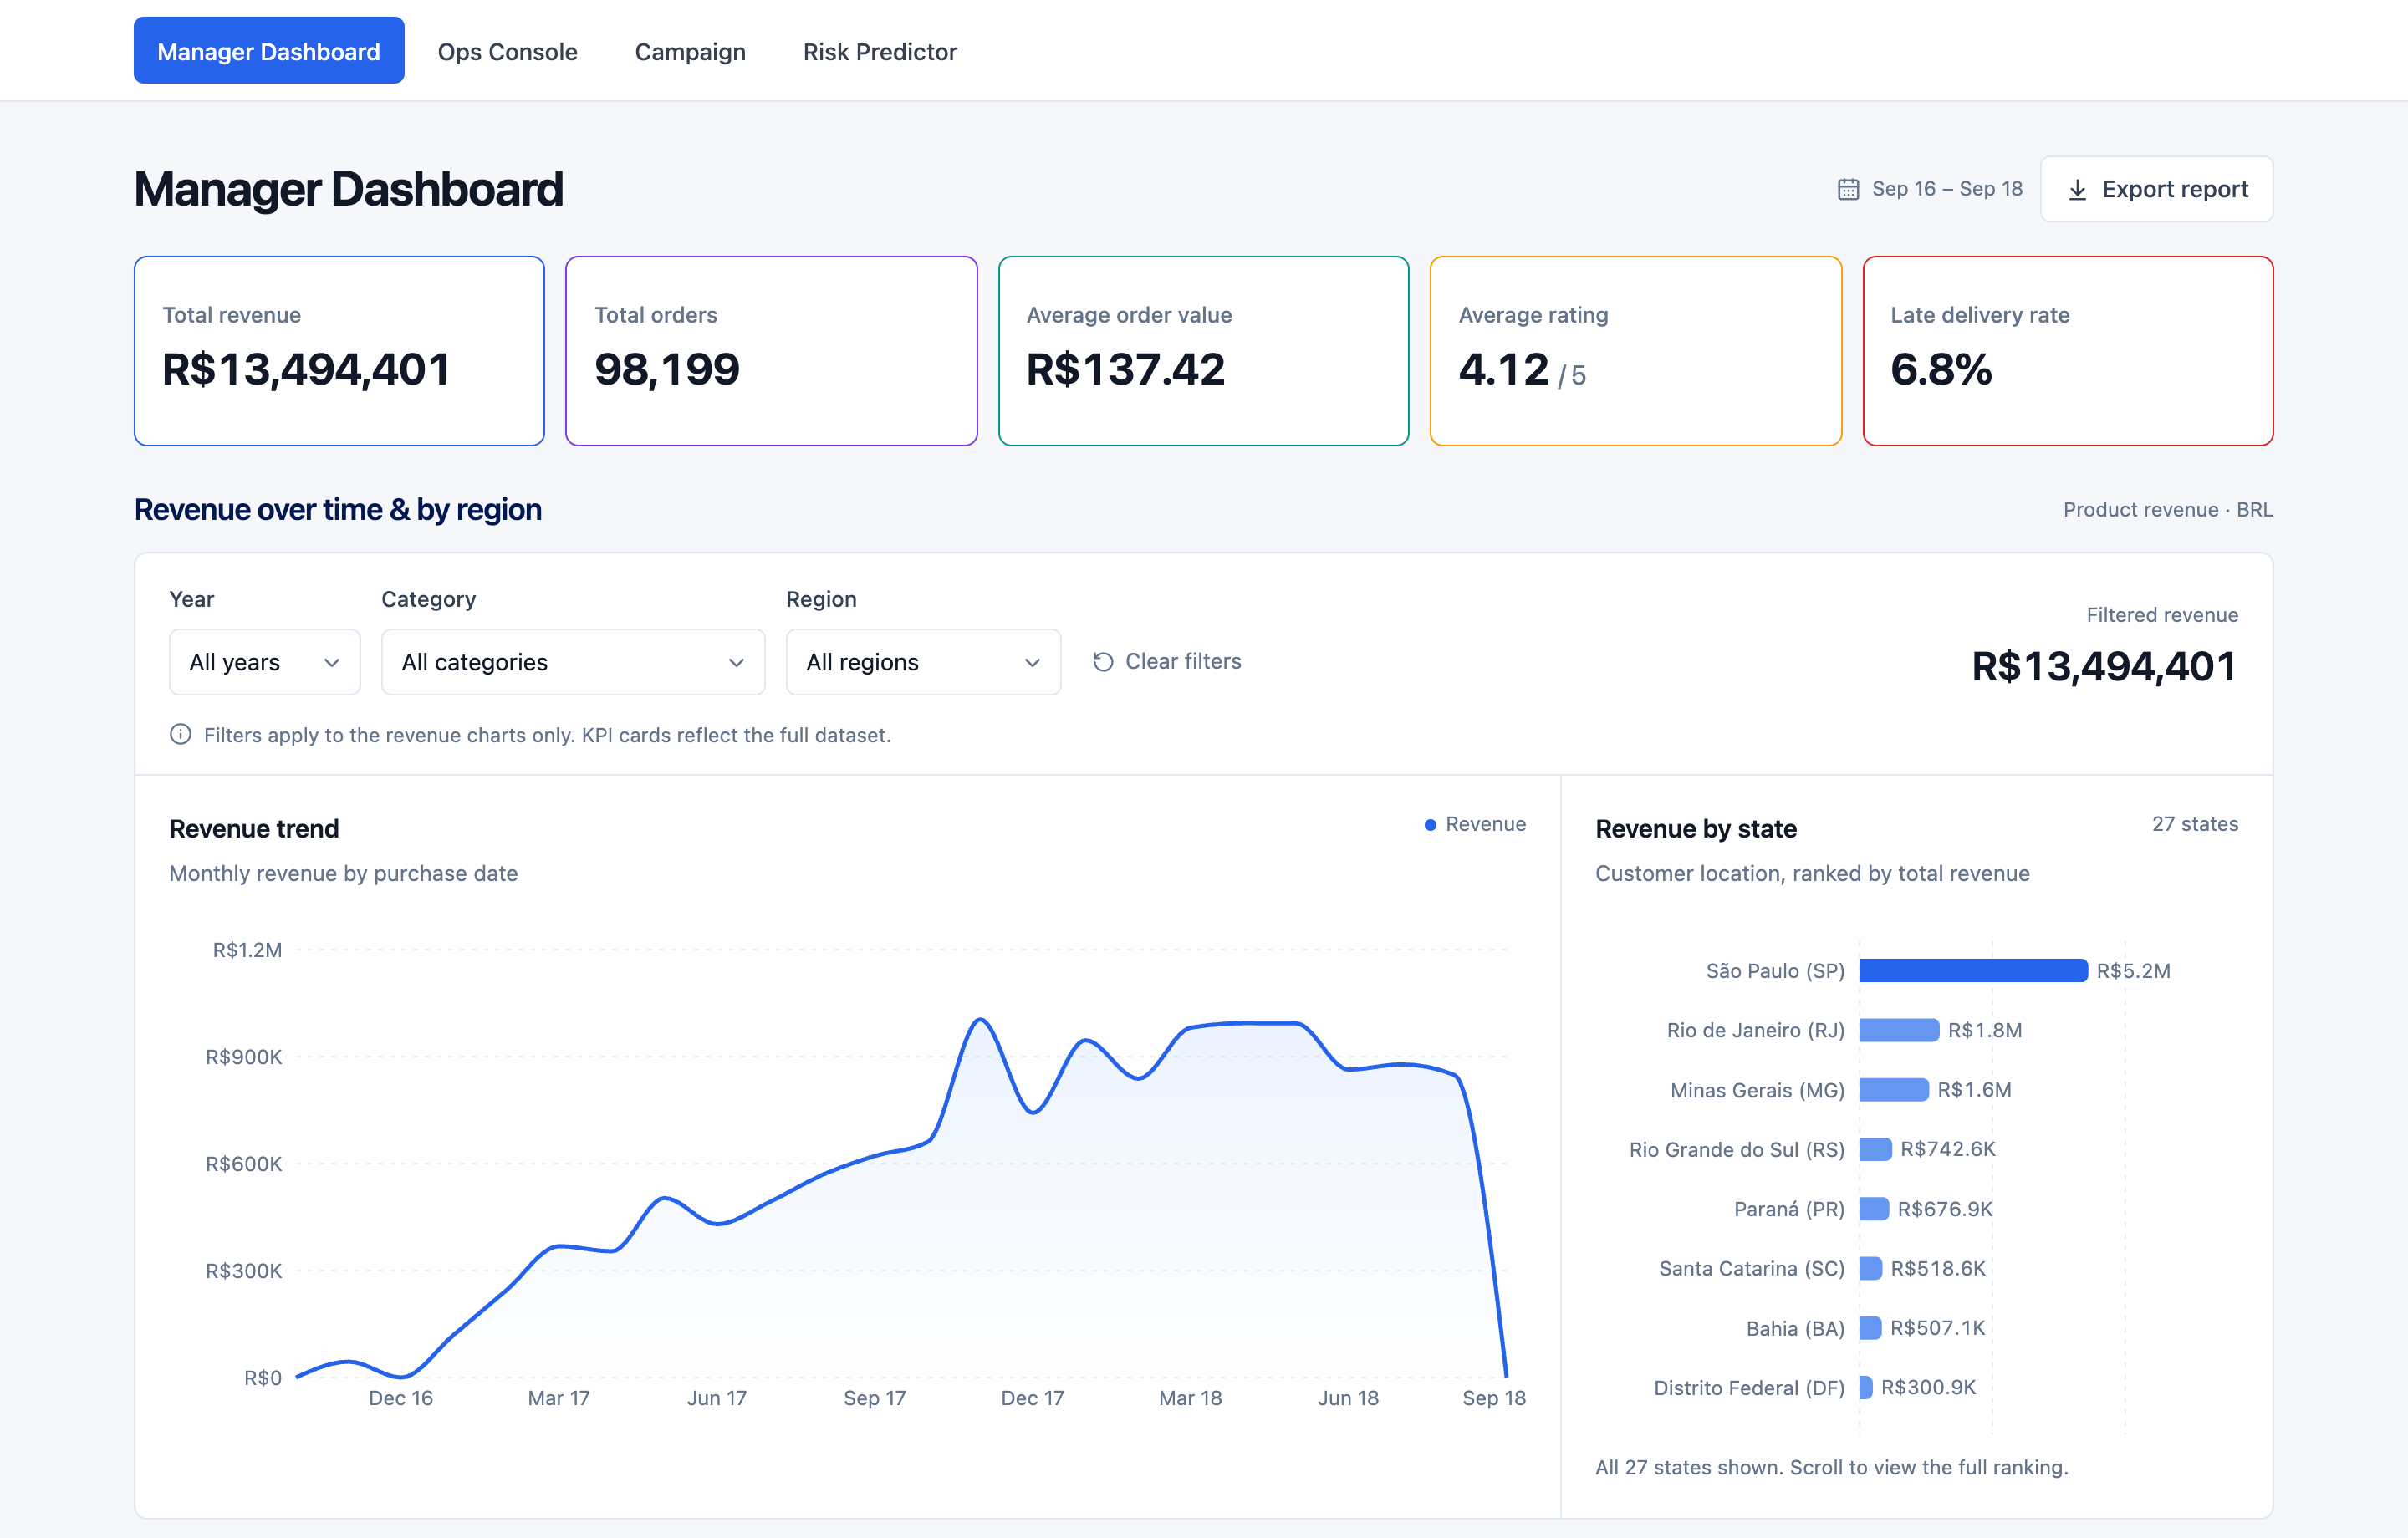
\includegraphics[width=0.85\textwidth]{Picture/ui_manager_overview.png}
\caption{Manager Dashboard: thanh tab trên cùng, thẻ KPI, doanh thu theo tháng và theo bang với bộ lọc năm/ngành/vùng}
\label{fig:ui-manager}
\end{figure}

\begin{figure}[H]
\centering
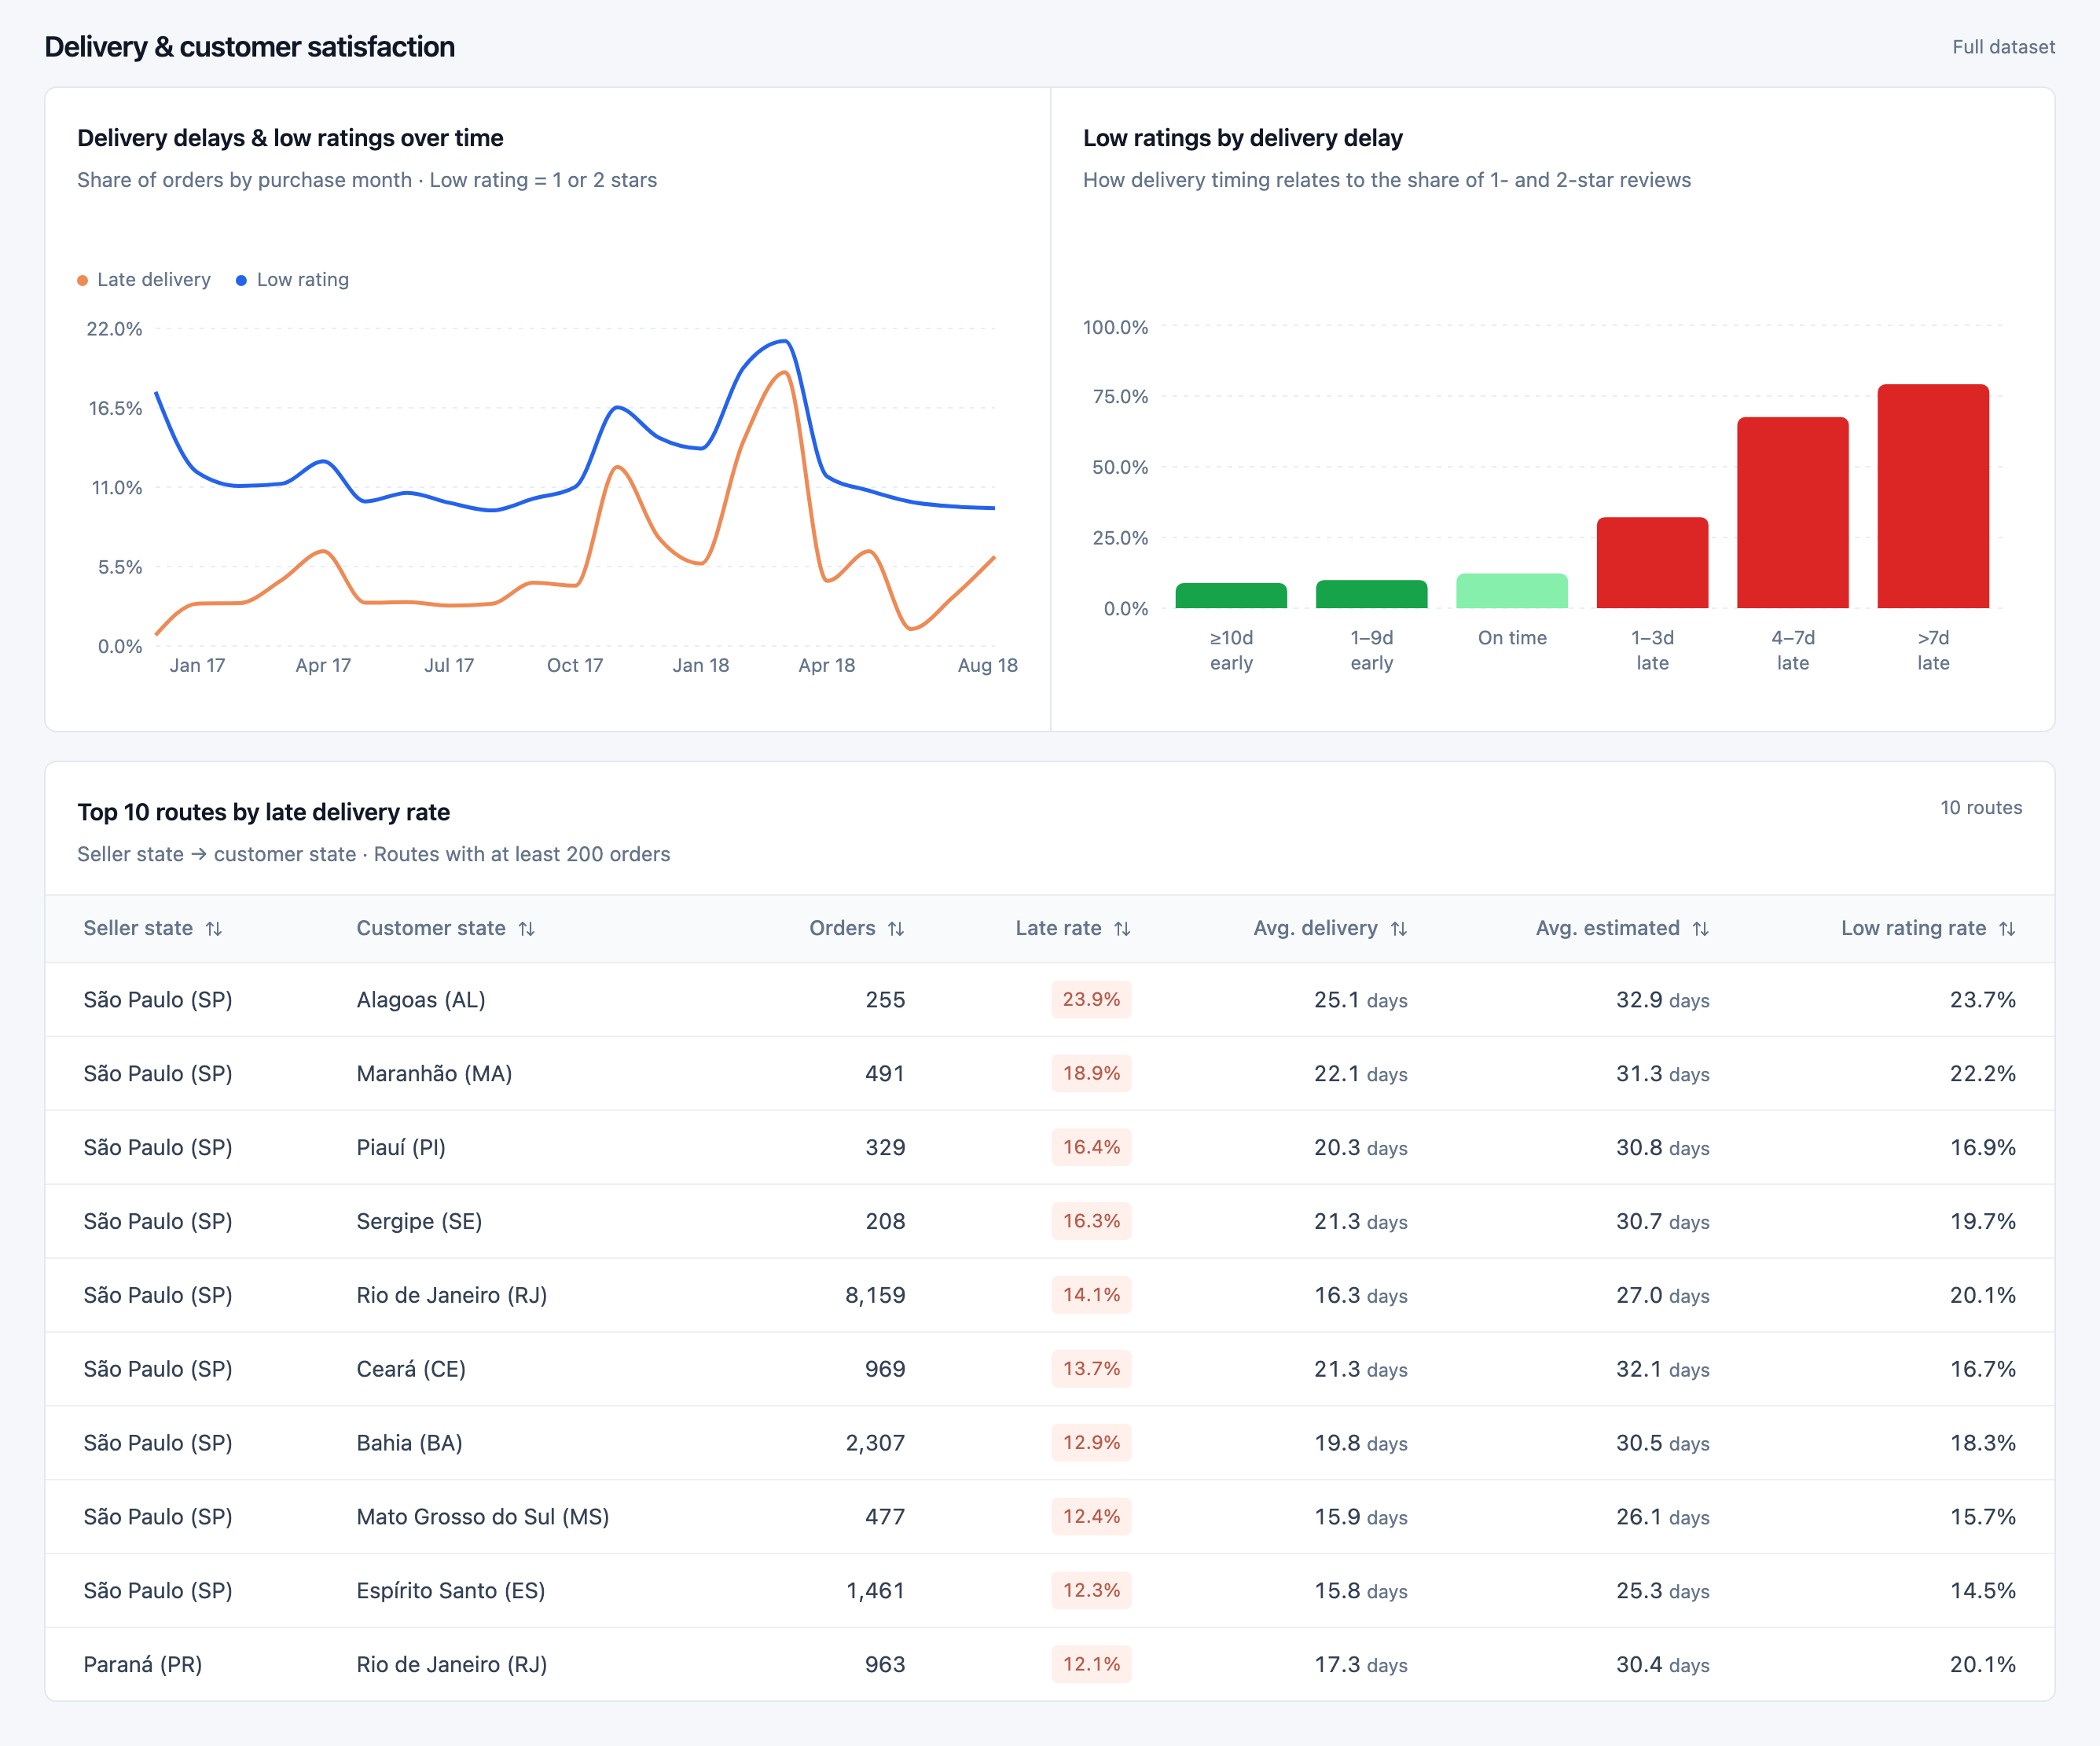
\includegraphics[width=0.85\textwidth]{Picture/ui_manager_delivery.png}
\caption{Manager Dashboard: phần giao hàng và mức độ hài lòng}
\label{fig:ui-delivery}
\end{figure}

\begin{figure}[H]
\centering
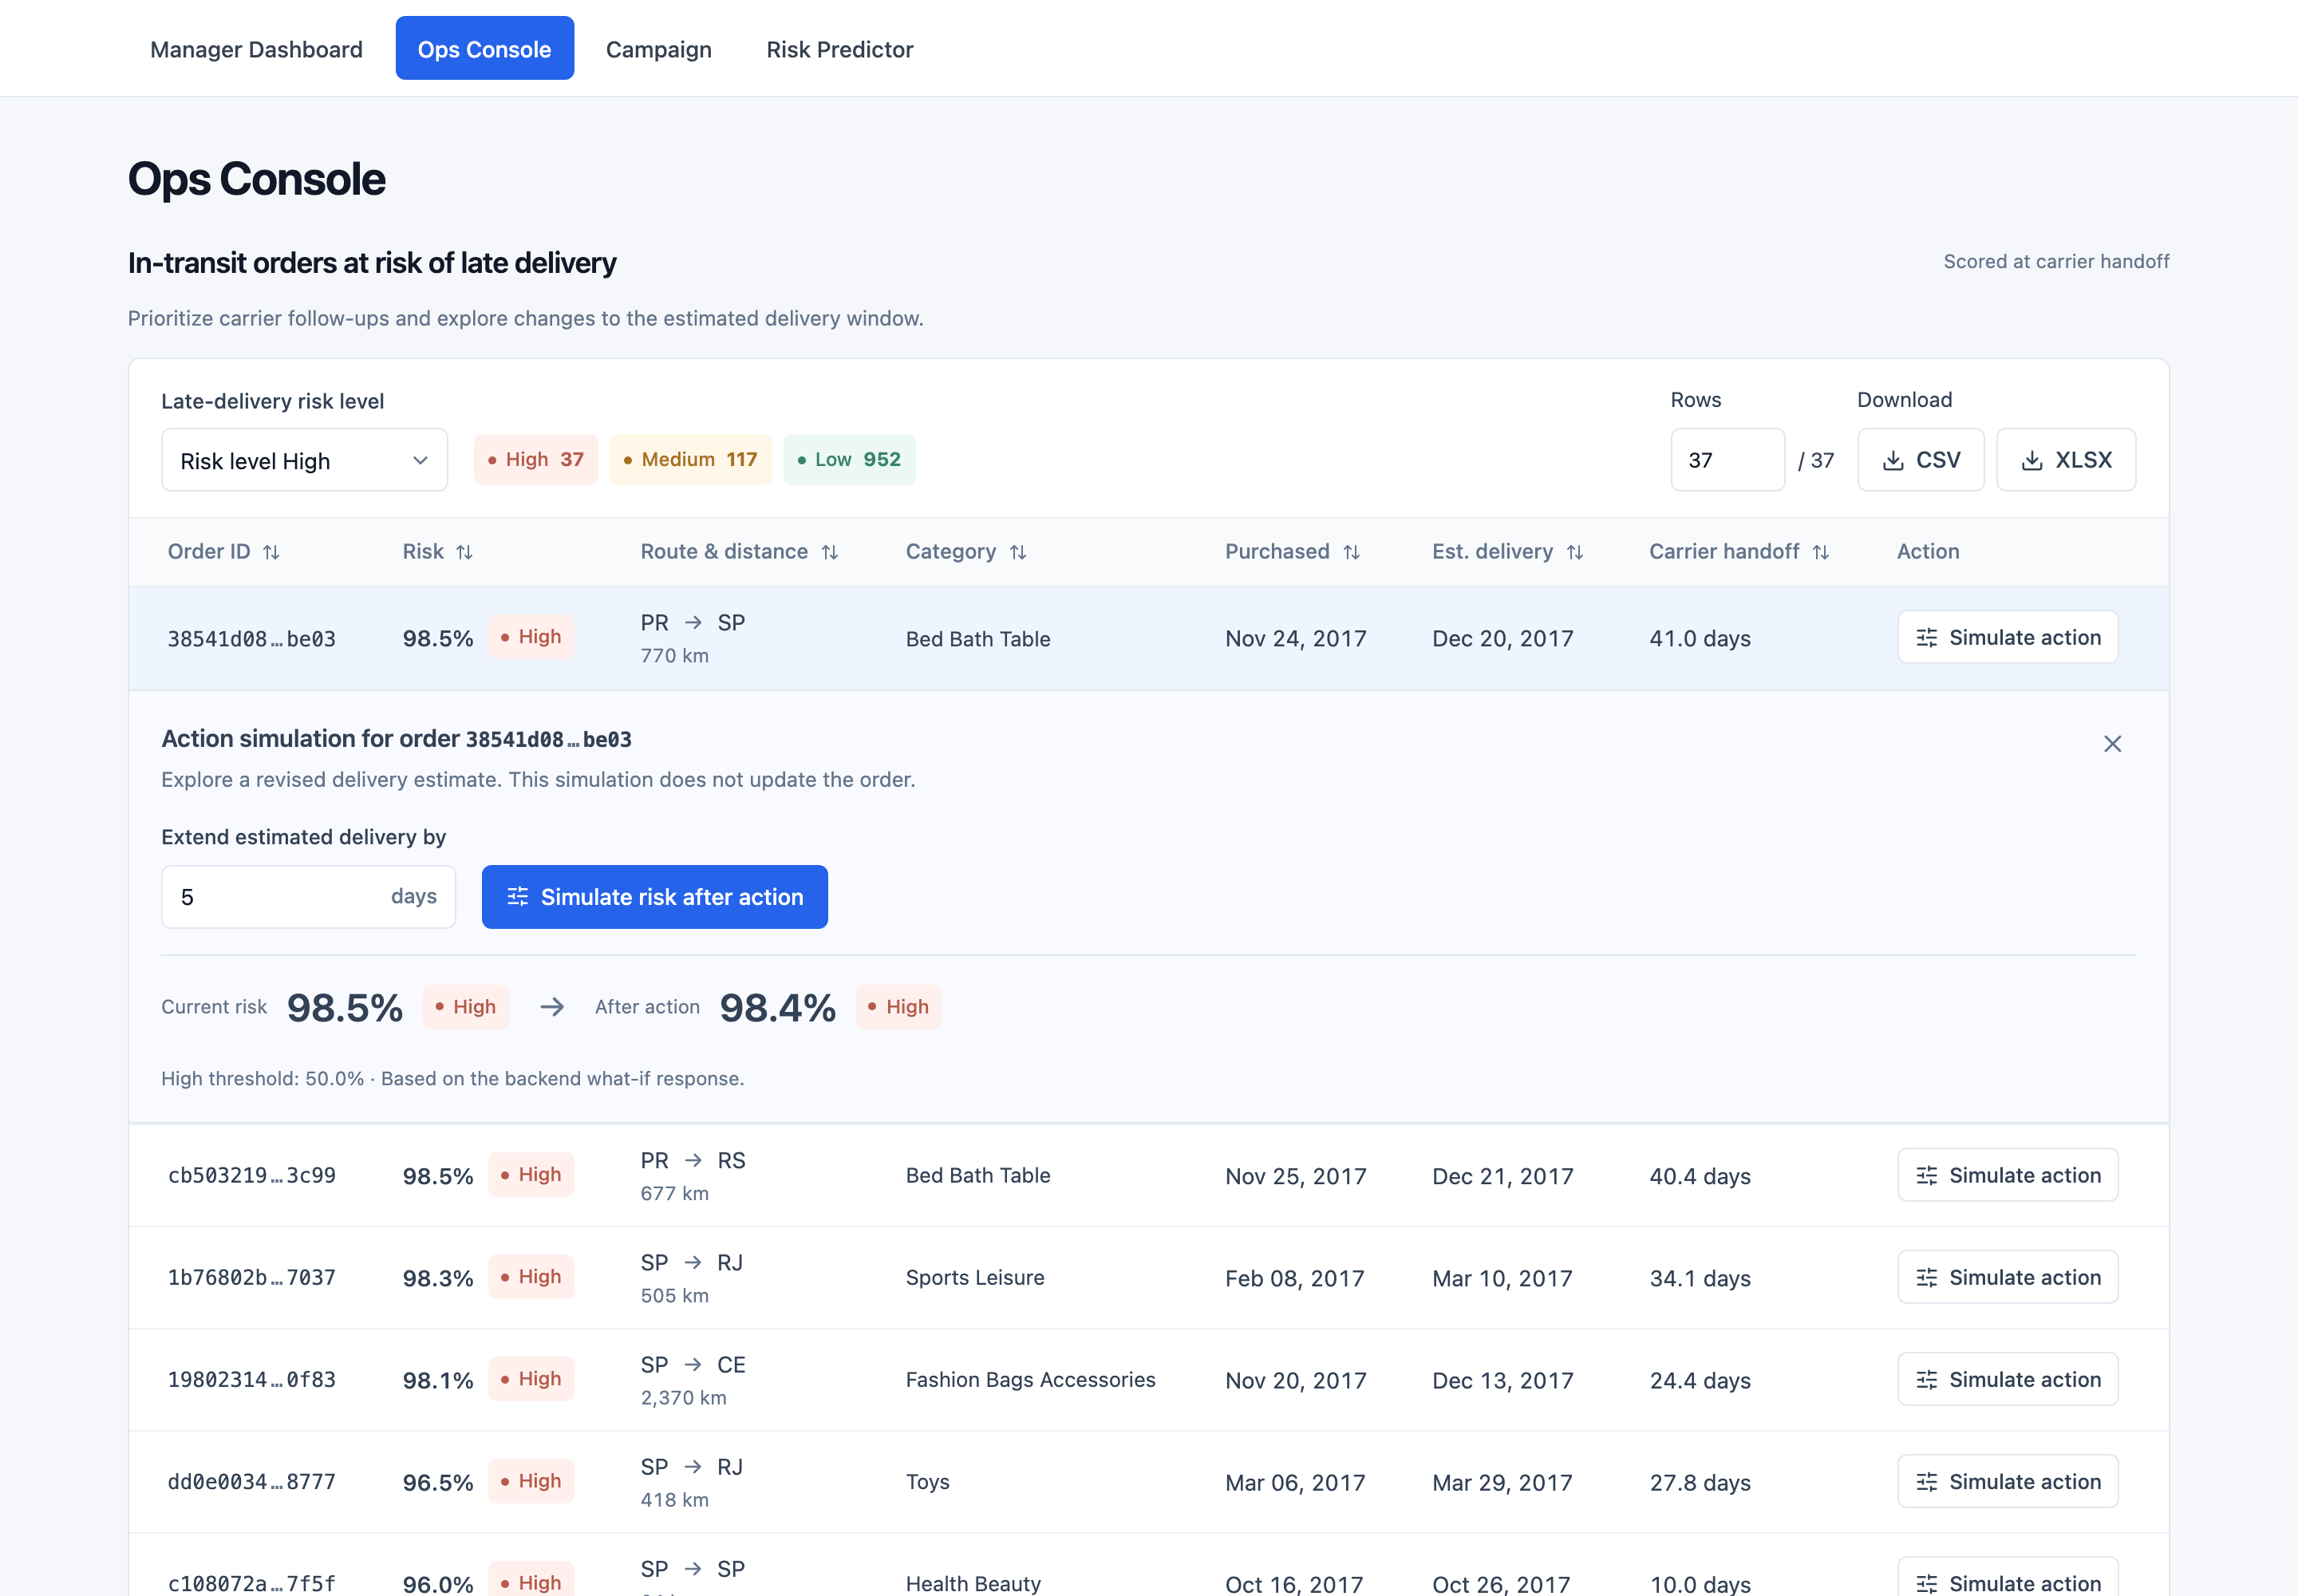
\includegraphics[width=0.85\textwidth]{Picture/ui_ops_late.png}
\caption{Ops Console: danh sách đơn đang vận chuyển có rủi ro giao trễ mức High kèm số đơn theo từng mức, ô chọn số dòng, nút tải CSV/XLSX và nút Simulate action}
\label{fig:ui-ops-late}
\end{figure}

\begin{figure}[H]
\centering
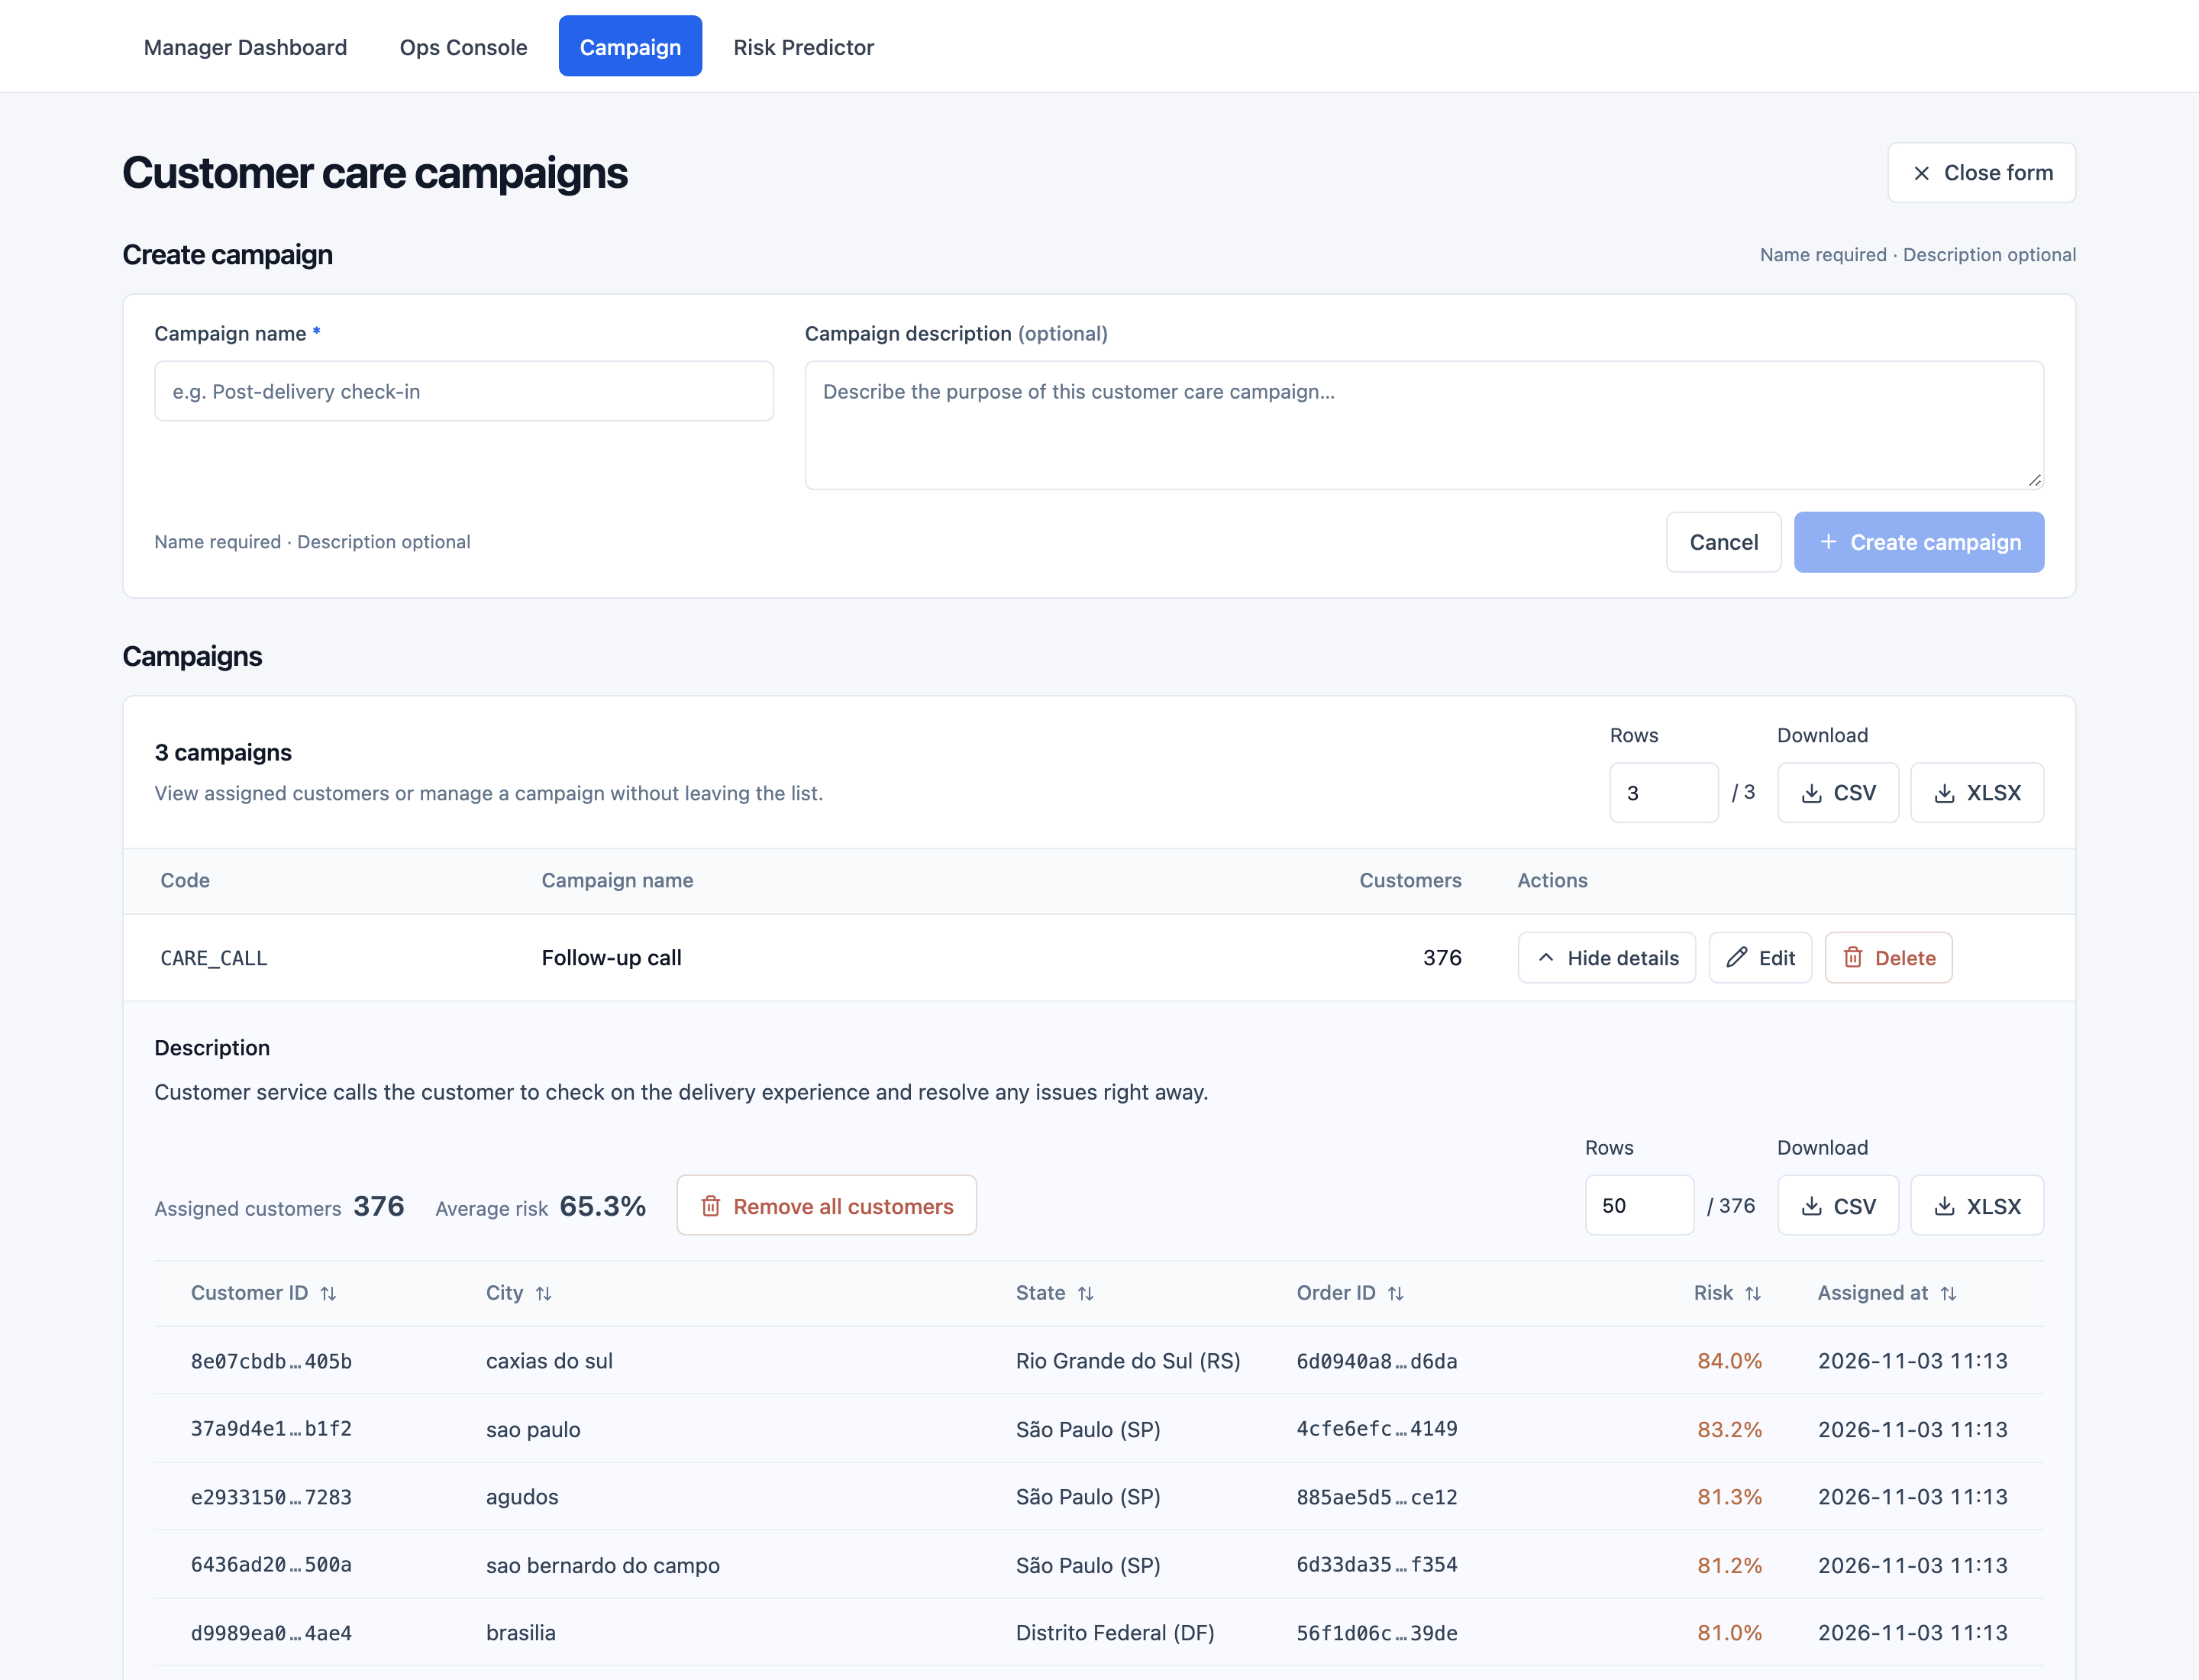
\includegraphics[width=0.85\textwidth]{Picture/ui_campaign.png}
\caption{Màn hình Campaign: danh sách chiến dịch, form thêm mới, phần chi tiết gồm mô tả và khách đã gắn}
\label{fig:ui-campaign}
\end{figure}

\begin{figure}[H]
\centering
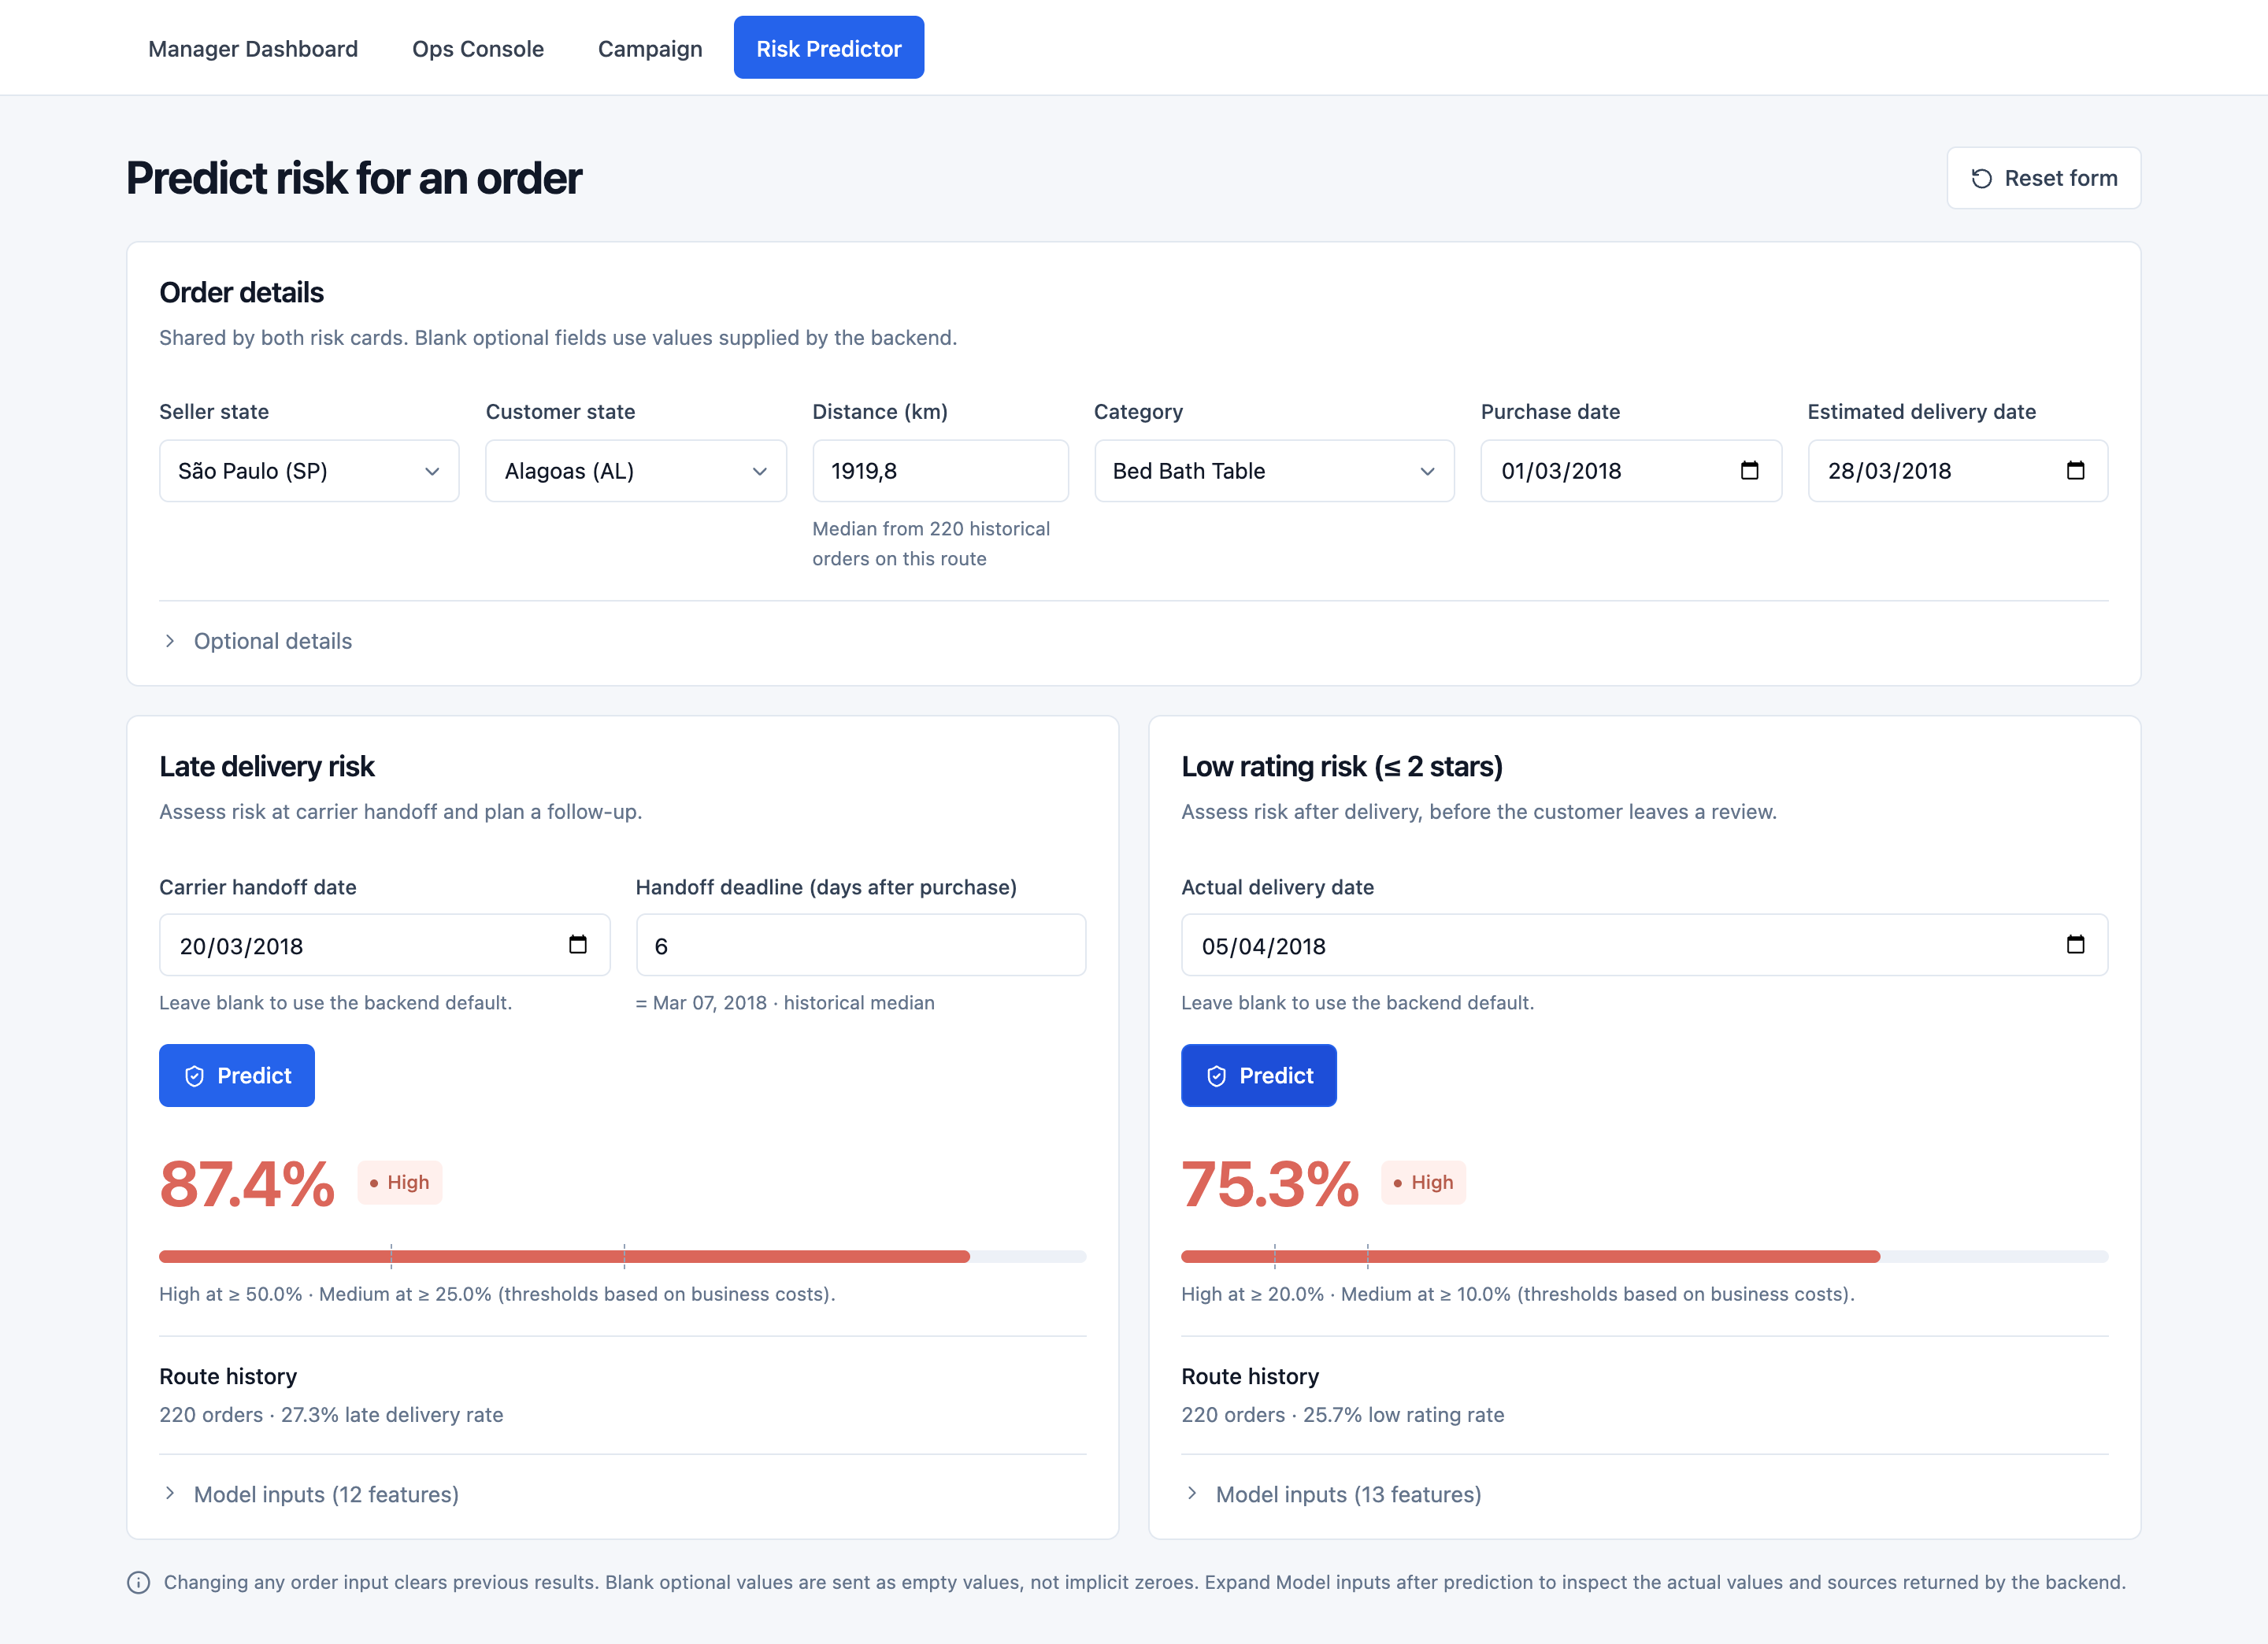
\includegraphics[width=0.85\textwidth]{Picture/ui_predict.png}
\caption{Risk Predictor: đơn giả định tuyến SP $\to$ AL, hẹn giao 27 ngày, người bán bàn giao vào
ngày thứ 19 (rủi ro trễ 87,4\%); nếu giao tới khách trễ 8 ngày thì rủi ro đánh giá thấp 75,3\%}
\label{fig:ui-predict}
\end{figure}

\subsection{Luồng dữ liệu đầu-cuối}
\hspace{1cm}
Hình~\ref{fig:sequence} minh họa luồng xử lý một yêu cầu điển hình từ Manager Dashboard: (1)
người dùng chọn khoảng thời gian trên dashboard; (2) frontend gọi API
\texttt{GET /dashboard/\allowbreak revenue-trend}; (3) backend-api truy vấn \texttt{mv\_revenue\_by\_month\_category}
trên kho dữ liệu; (4) kết quả trả về và được trực quan hóa dưới dạng biểu đồ.

\begin{figure}[H]
\centering
\begin{tikzpicture}[
    actor/.style={draw, rounded corners, fill=black!5, minimum width=2.8cm,
                  minimum height=1.2cm, font=\small, align=center},
    lbl/.style={font=\scriptsize, align=center},
    arr/.style={-{Stealth[length=2mm]}, thick}
]
\node[actor] (fe) at (0,0) {Manager\\Dashboard};
\node[actor] (be) at (7,0) {Backend API\\(BFF)};
\node[actor] (dw) at (14,0) {Kho dữ liệu\\(OLAP view)};

\draw[arr] ([yshift=5pt]fe.east) -- node[above, lbl]{\texttt{GET /dashboard/revenue-trend}\\\texttt{?year=\&category=\&region=}}
    ([yshift=5pt]be.west);
\draw[arr] ([yshift=5pt]be.east) -- node[above, lbl]{\texttt{SELECT ... FROM}\\\texttt{mv\_revenue\_by\_}\\\texttt{month\_category}}
    ([yshift=5pt]dw.west);
\draw[arr] ([yshift=-8pt]dw.west) -- node[below, lbl]{Các dòng kết quả}
    ([yshift=-8pt]be.east);
\draw[arr] ([yshift=-8pt]be.west) -- node[below, lbl]{JSON}
    ([yshift=-8pt]fe.east);
\end{tikzpicture}
\caption{Luồng xử lý một yêu cầu truy vấn doanh thu từ dashboard}
\label{fig:sequence}
\end{figure}

\subsection{Nạp dữ liệu và vận hành thử nghiệm}
\hspace{1cm}
Môi trường demo được khởi tạo theo một trong hai cách: chạy
\texttt{bash scripts/seed\_db.sh} (tạo schema, Extract, Transform,
Load rồi chạy kiểm tra chất lượng, sau đó train mô hình trong container bằng
\texttt{POST /risk/retrain}), hoặc kích hoạt DAG \texttt{staging\_load} trên Airflow để
chuỗi \texttt{staging\_load} $\to$ \texttt{dw\_load} $\to$ \texttt{dss\_batch} tự chạy. Các
dịch vụ backend khởi động bằng \texttt{docker compose up -d}, với Airflow UI tại cổng 8080,
DSS service tại cổng 8001, backend API tại cổng 8000 và PostgreSQL tại cổng 5433; frontend
chạy riêng bằng \texttt{npm run dev} tại cổng 5173.

\textbf{Kết quả vận hành.} Kích hoạt \texttt{staging\_load} trên Airflow, cả ba DAG chạy thành
công nối tiếp nhau, mỗi DAG dưới một phút. Chạy lại không làm thay đổi số dòng (98.666 đơn trong
\texttt{FACT\_ORDER\_FULFILLMENT}, 96.355 phiên bản khách hàng, 38.229 điểm rủi ro) và chỉ số
mô hình giữ nguyên, xác nhận pipeline idempotent và kết quả lặp lại được.

\textbf{Lưu ý về phiên bản thư viện.} File mô hình (\texttt{dss/models/*.pkl}) phải được huấn
luyện bằng cùng phiên bản scikit-learn với container \texttt{dss} (1.9.1); mô hình train trên
máy với phiên bản khác không nạp được trong container. Vì vậy mô hình luôn được huấn luyện lại
bên trong container qua \texttt{POST /risk/retrain} (DAG \texttt{dss\_batch}).

\textbf{Tài liệu trình bày và tái lập kết quả.}
\begin{itemize}
    \item \texttt{dss/notebooks/\allowbreak risk\_models.ipynb}: notebook đi lại từng bước của
          \texttt{dss/risk/\allowbreak train.py} -- đọc dữ liệu từ kho, khám phá dữ liệu, đặc trưng và chống
          leakage, chia theo thời gian, huấn luyện HGB và baseline, ngưỡng theo chi phí, đường
          precision--recall, feature importance, thí nghiệm chấm điểm sớm và drift, what-if. Notebook
          gọi chính các hàm của project và chỉ đọc kho dữ liệu, nên số liệu khớp với hệ thống
          và với Chương~6.
    \item \texttt{report/scripts/make\_figures.py}: vẽ lại các biểu đồ của Chương~6 (tỷ lệ trễ
          theo tháng, đường precision--recall, feature importance) trực tiếp từ kho dữ liệu sau
          mỗi lần huấn luyện lại.
\end{itemize}


\newpage
\section{KẾT QUẢ}\label{sec:ket-qua}
\hspace{1cm}

Môi trường demo được khởi tạo theo một trong hai cách: chạy
\texttt{bash scripts/seed\_db.sh} (tạo schema, Extract, Transform,
Load rồi chạy kiểm tra chất lượng, sau đó train mô hình trong container bằng
\texttt{POST /risk/retrain}), hoặc kích hoạt DAG \texttt{staging\_load} trên Airflow để
chuỗi \texttt{staging\_load} $\to$ \texttt{dw\_load} $\to$ \texttt{dss\_batch} tự chạy. 
% Các
% dịch vụ backend khởi động bằng \texttt{docker compose up -d}, với Airflow UI tại cổng 8080,
% DSS service tại cổng 8001, backend API tại cổng 8000 và PostgreSQL tại cổng 5433; frontend
% chạy riêng bằng \texttt{npm run dev} tại cổng 5173.

\textbf{Kết quả:} Kích hoạt \texttt{staging\_load} trên Airflow, cả ba DAG chạy thành
công nối tiếp nhau, mỗi DAG dưới một phút. Chạy lại không làm thay đổi số dòng (98.666 đơn trong
\texttt{FACT\_ORDER\_FULFILLMENT}, 96.355 phiên bản khách hàng, 38.229 điểm rủi ro) và chỉ số
mô hình giữ nguyên, xác nhận pipeline idempotent và kết quả lặp lại được.

% \textbf{Lưu ý về phiên bản thư viện.} File mô hình (\texttt{dss/models/*.pkl}) phải được huấn
% luyện bằng cùng phiên bản scikit-learn với container \texttt{dss} (1.9.1); mô hình train trên
% máy với phiên bản khác không nạp được trong container. Vì vậy mô hình luôn được huấn luyện lại
% bên trong container qua \texttt{POST /risk/retrain} (DAG \texttt{dss\_batch}).


% \textbf{Tài liệu trình bày và tái lập kết quả.}
% \begin{itemize}
%     \item \texttt{dss/notebooks/\allowbreak risk\_models.ipynb}: notebook đi lại từng bước của
%           \texttt{dss/risk/\allowbreak train.py} -- đọc dữ liệu từ kho, khám phá dữ liệu, đặc trưng và chống
%           leakage, chia theo thời gian, huấn luyện HGB và baseline, ngưỡng theo chi phí, đường
%           precision--recall, feature importance, thí nghiệm chấm điểm sớm và drift, what-if. Notebook
%           gọi chính các hàm của project và chỉ đọc kho dữ liệu, nên số liệu khớp với hệ thống
%           và với Chương~6.
%     \item \texttt{report/scripts/make\_figures.py}: vẽ lại các biểu đồ của Chương~6 (tỷ lệ trễ
%           theo tháng, đường precision--recall, feature importance) trực tiếp từ kho dữ liệu sau
%           mỗi lần huấn luyện lại.
% \end{itemize}


Frontend gồm bốn màn hình chọn qua thanh tab: 
\begin{itemize}
      \item \textbf{Manager Dashboard} (KPI, doanh thu theo tháng và theo bang có bộ lọc năm/ngành/vùng, giao hàng và mức độ hài lòng, sản phẩm doanh thu cao nhất/thấp nhất)
      \item \textbf{Ops Console} (đơn có rủi ro giao trễ hoặc đánh giá thấp, \textit{Simulate action} mô phỏng kéo dài ngày hẹn giao, gắn khách vào chiến dịch)
      \item \textbf{Campaign} (quản lý chiến dịch và khách đã gắn)
      \item \textbf{Risk Predictor} (chấm điểm rủi ro cho một đơn tự nhập, Mục~\ref{sec:dss-whatif})
\end{itemize}
Các danh sách đều cho phép chọn số dòng và tải về tệp \texttt{.csv}/\texttt{.xlsx}.

Hình~\ref{fig:ui-manager}--\ref{fig:ui-predict} là ảnh chụp bốn màn hình khi chạy với dữ liệu thật.

\begin{figure}[H]
\centering
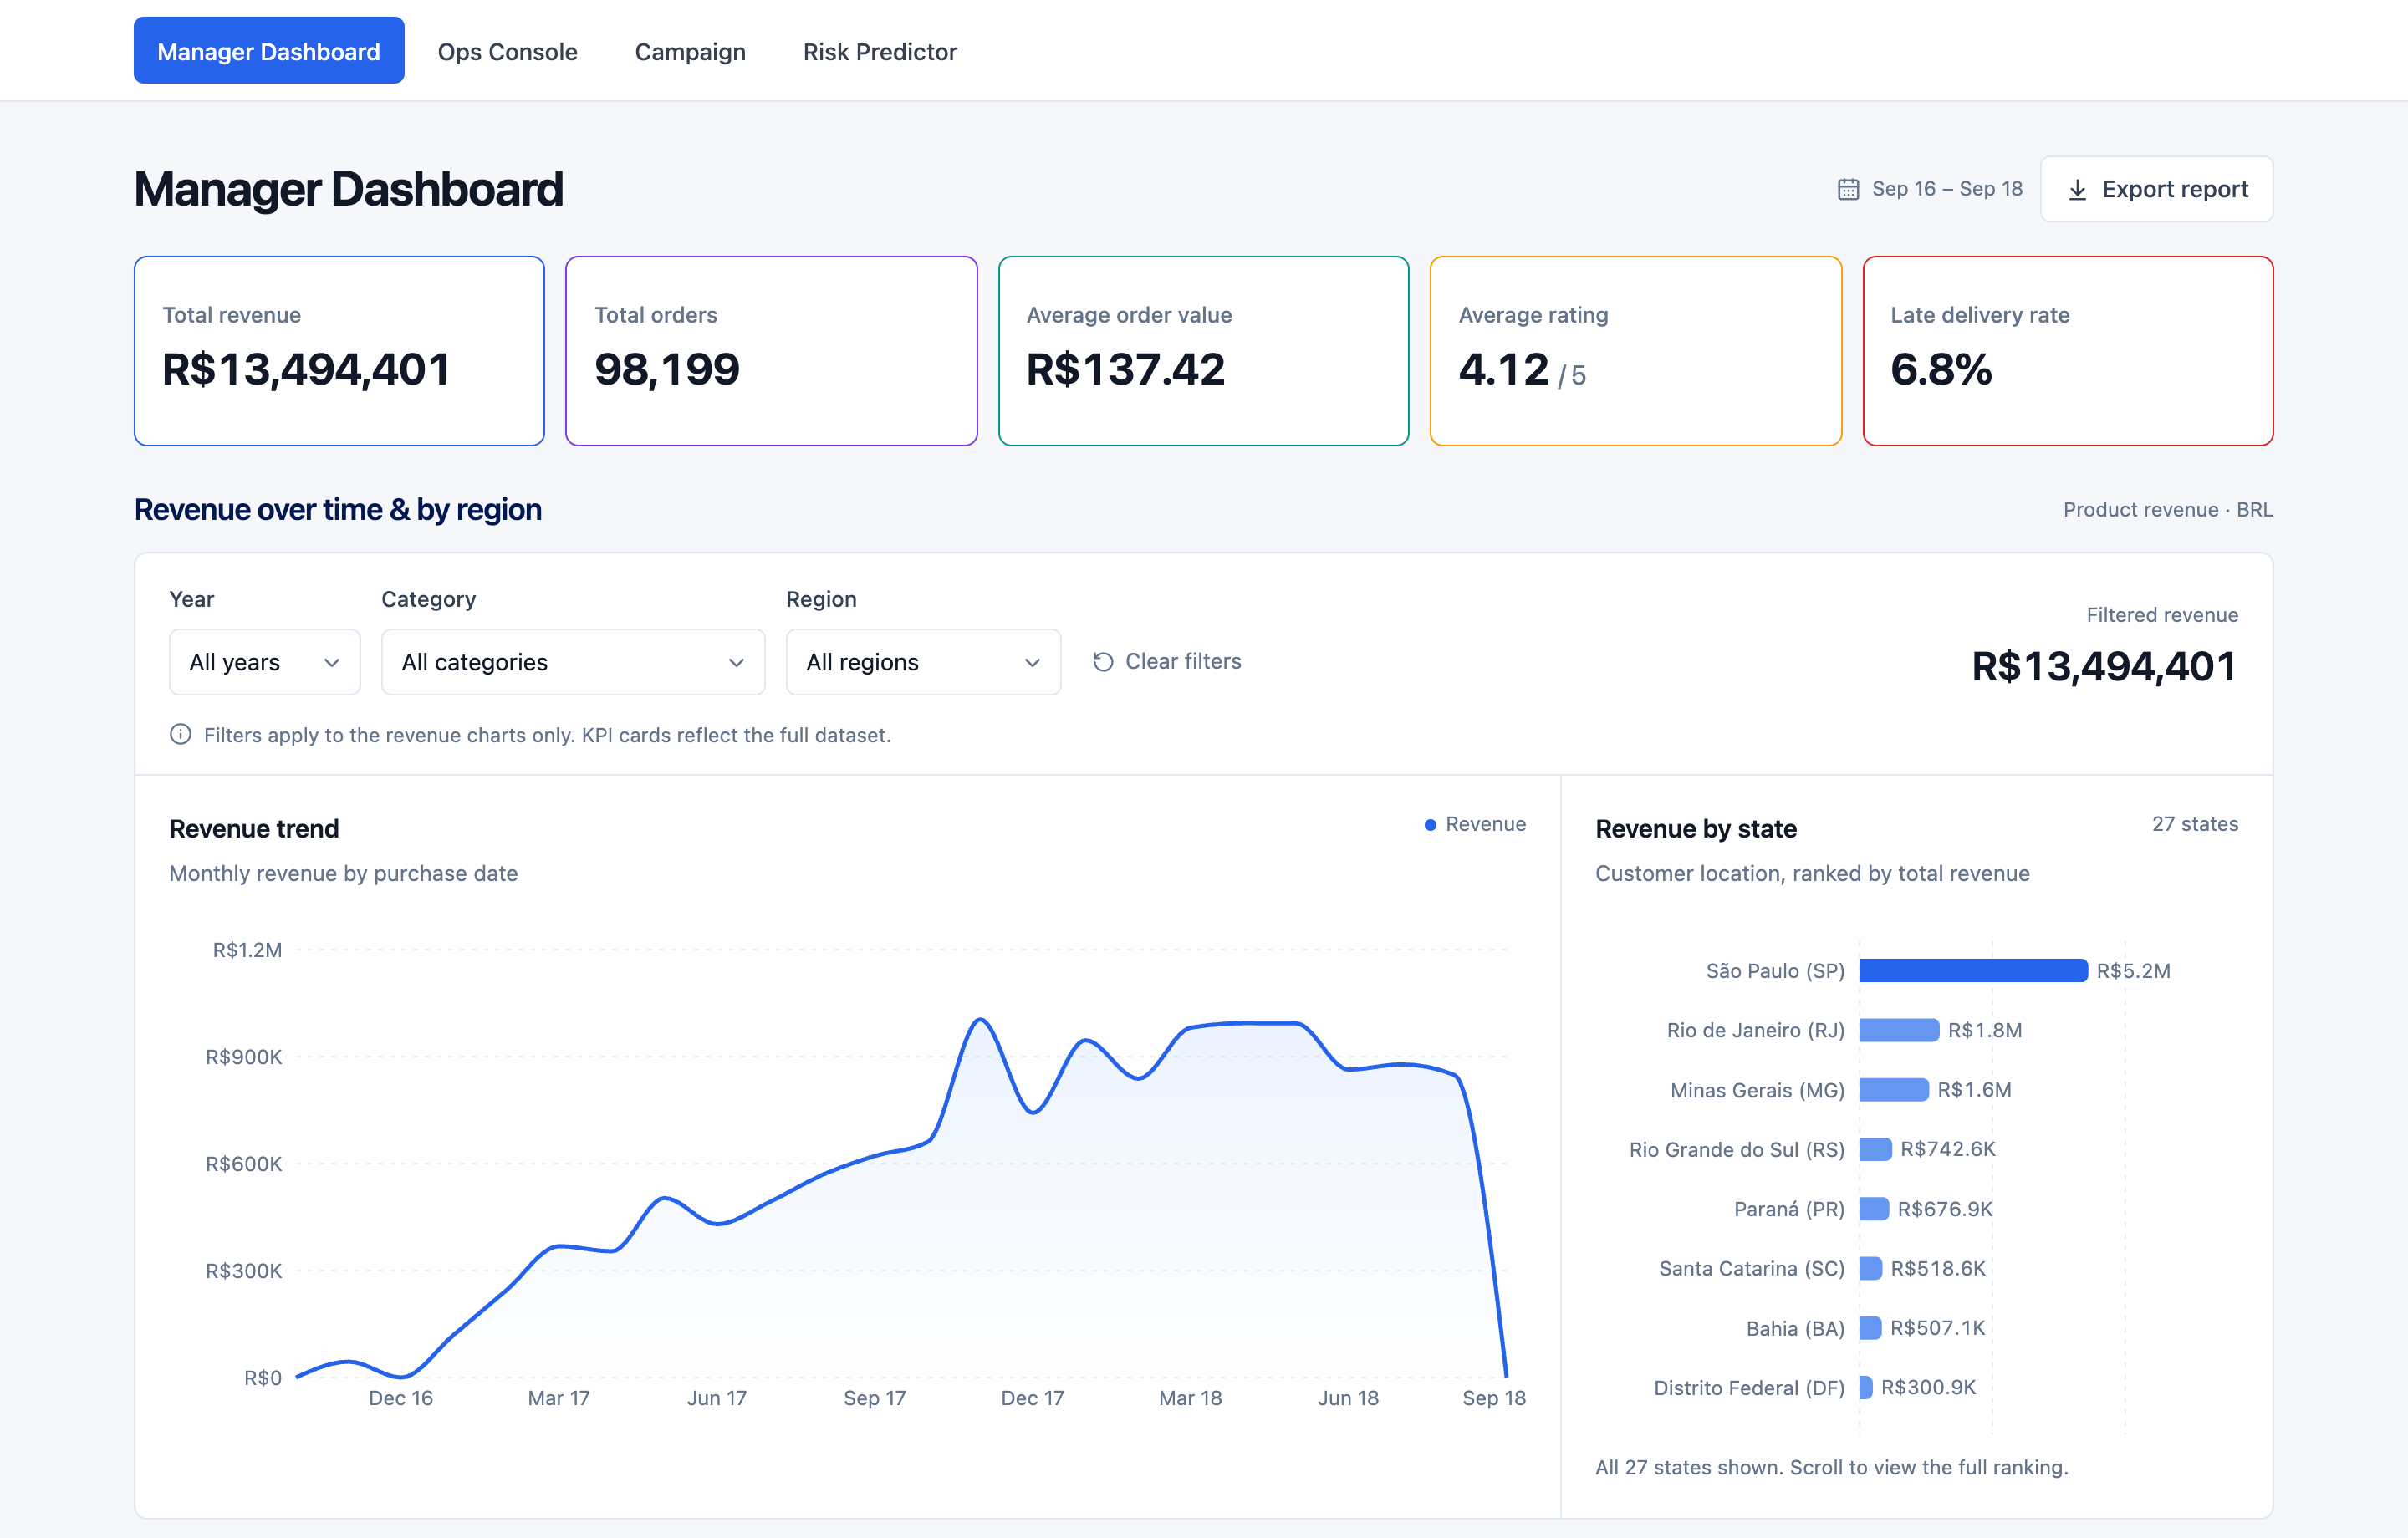
\includegraphics[width=0.75\textwidth]{Picture/ui_manager_overview.png}
\caption{Manager Dashboard: thanh tab trên cùng, thẻ KPI, doanh thu theo tháng và theo bang với bộ lọc năm/ngành/vùng}
\label{fig:ui-manager}
\end{figure}

\begin{figure}[H]
\centering
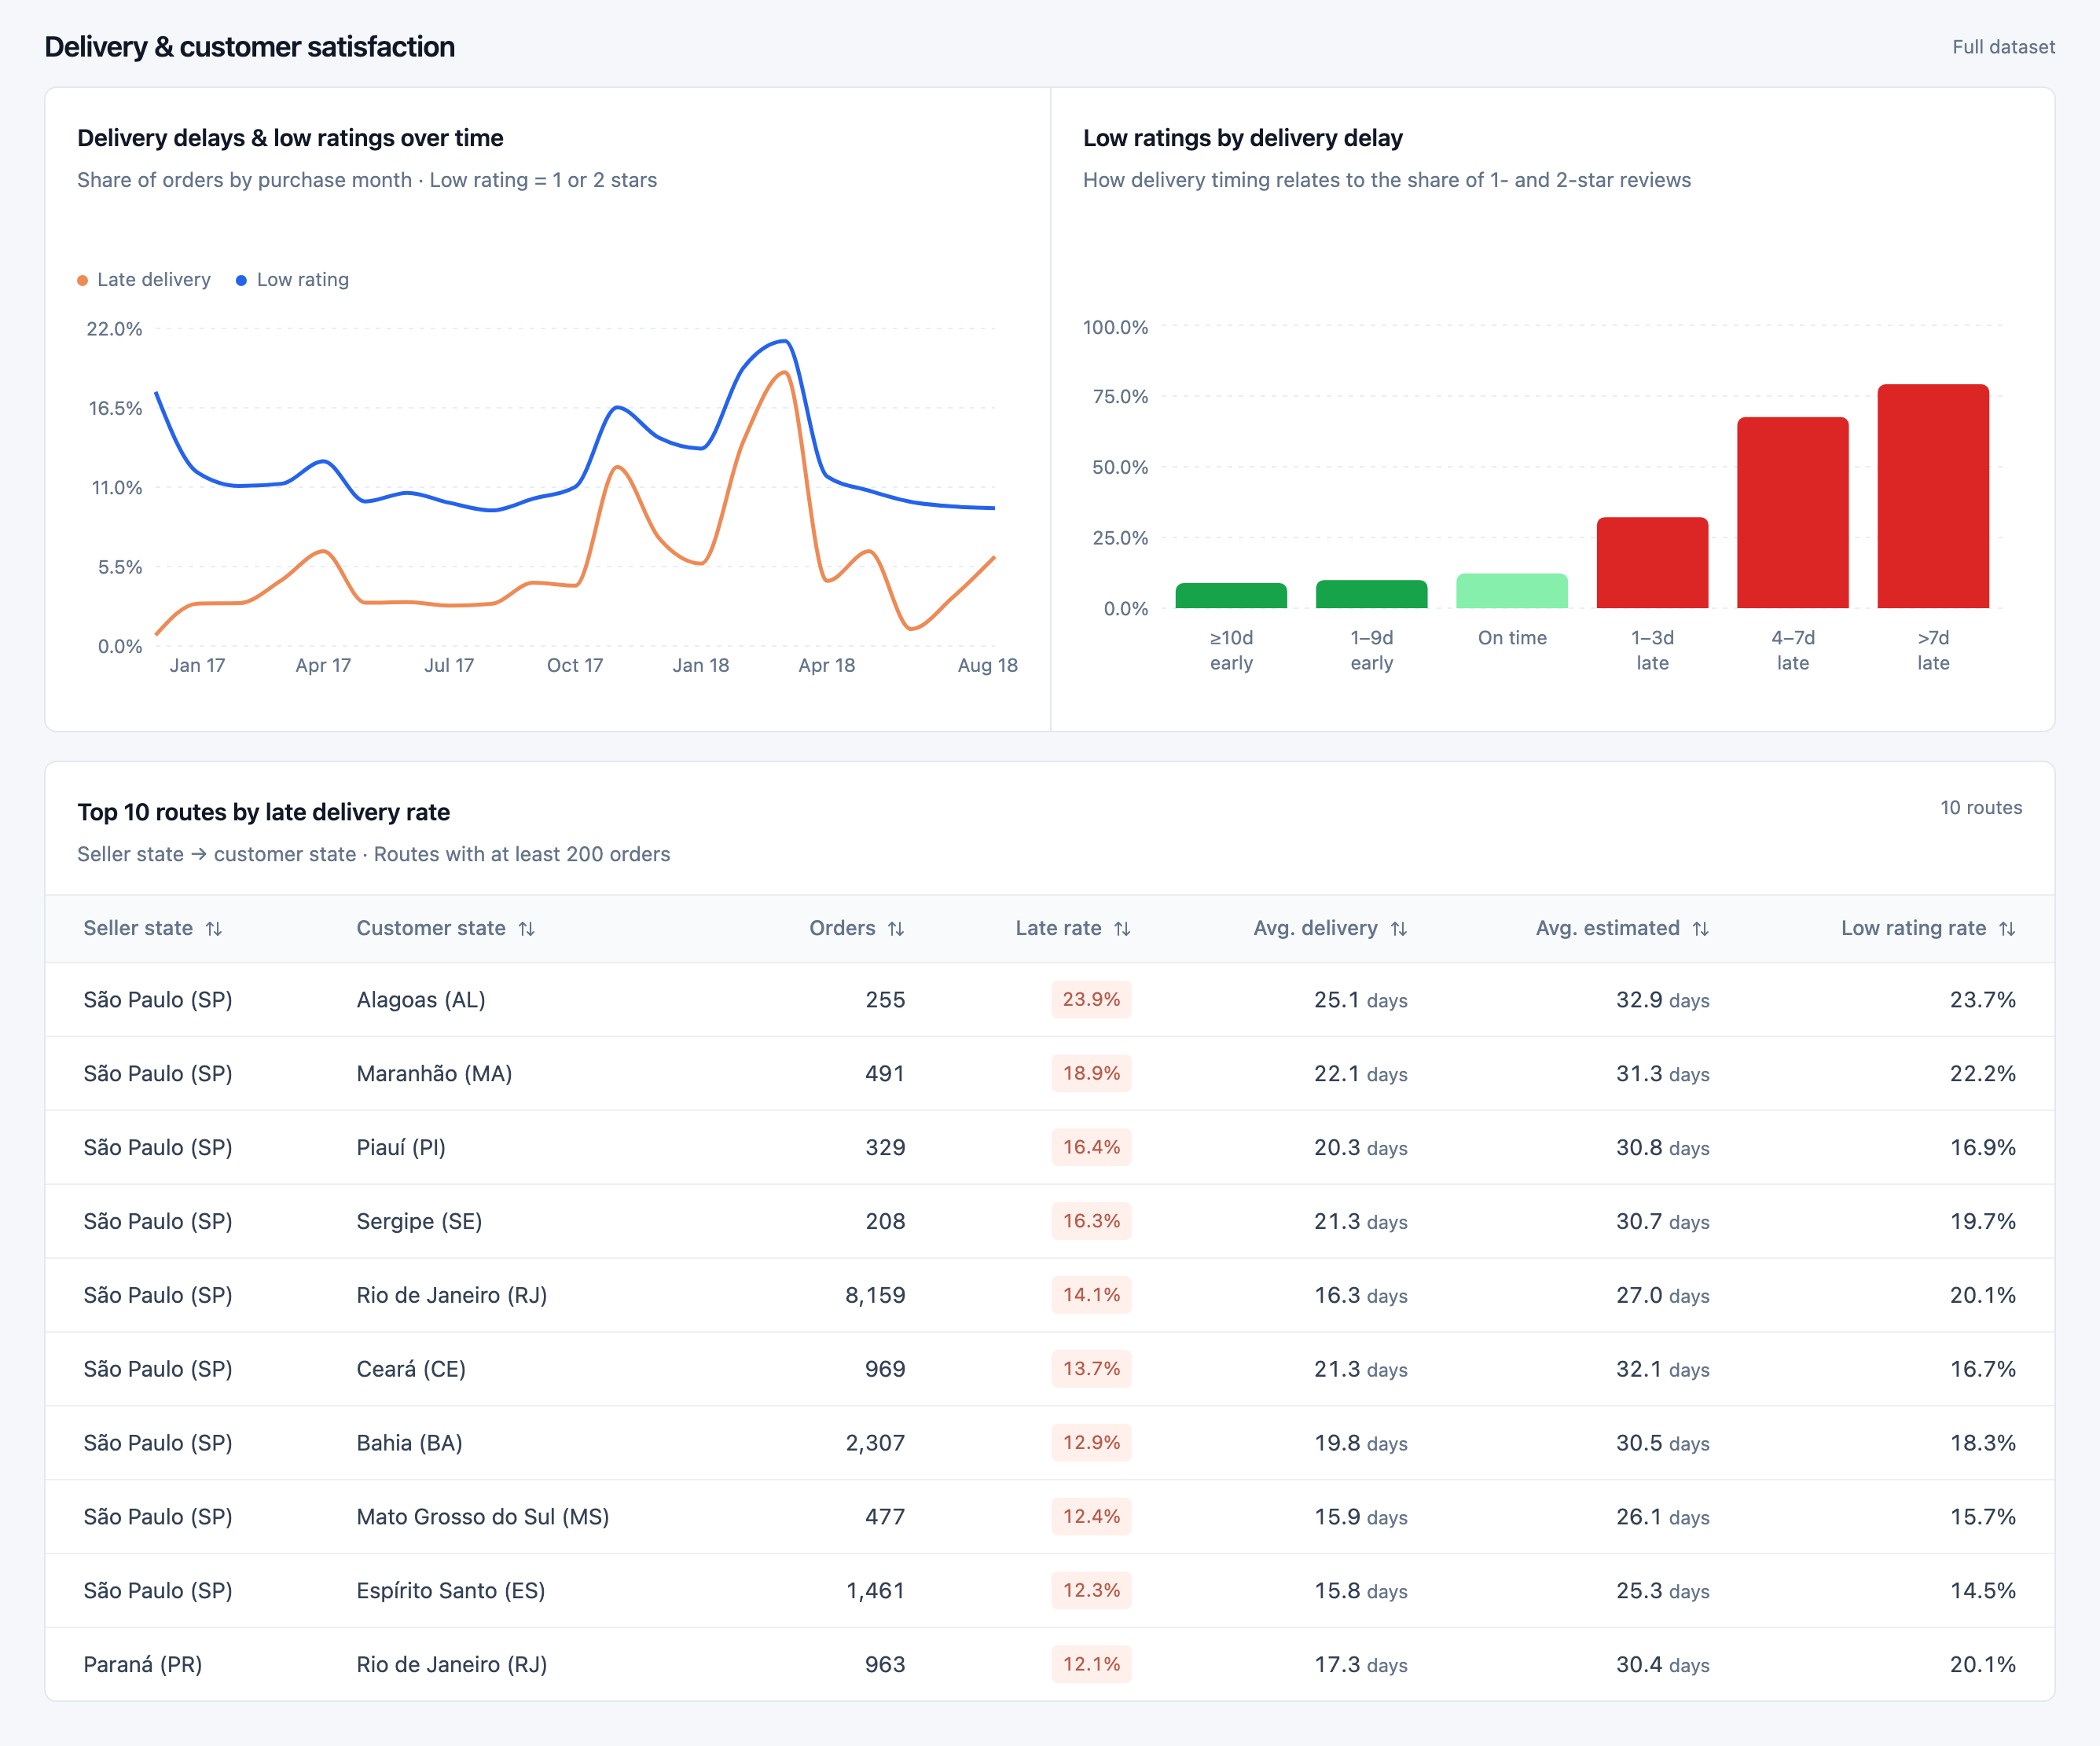
\includegraphics[width=0.75\textwidth]{Picture/ui_manager_delivery.png}
\caption{Manager Dashboard: phần giao hàng và mức độ hài lòng}
\label{fig:ui-delivery}
\end{figure}

\begin{figure}[H]
\centering
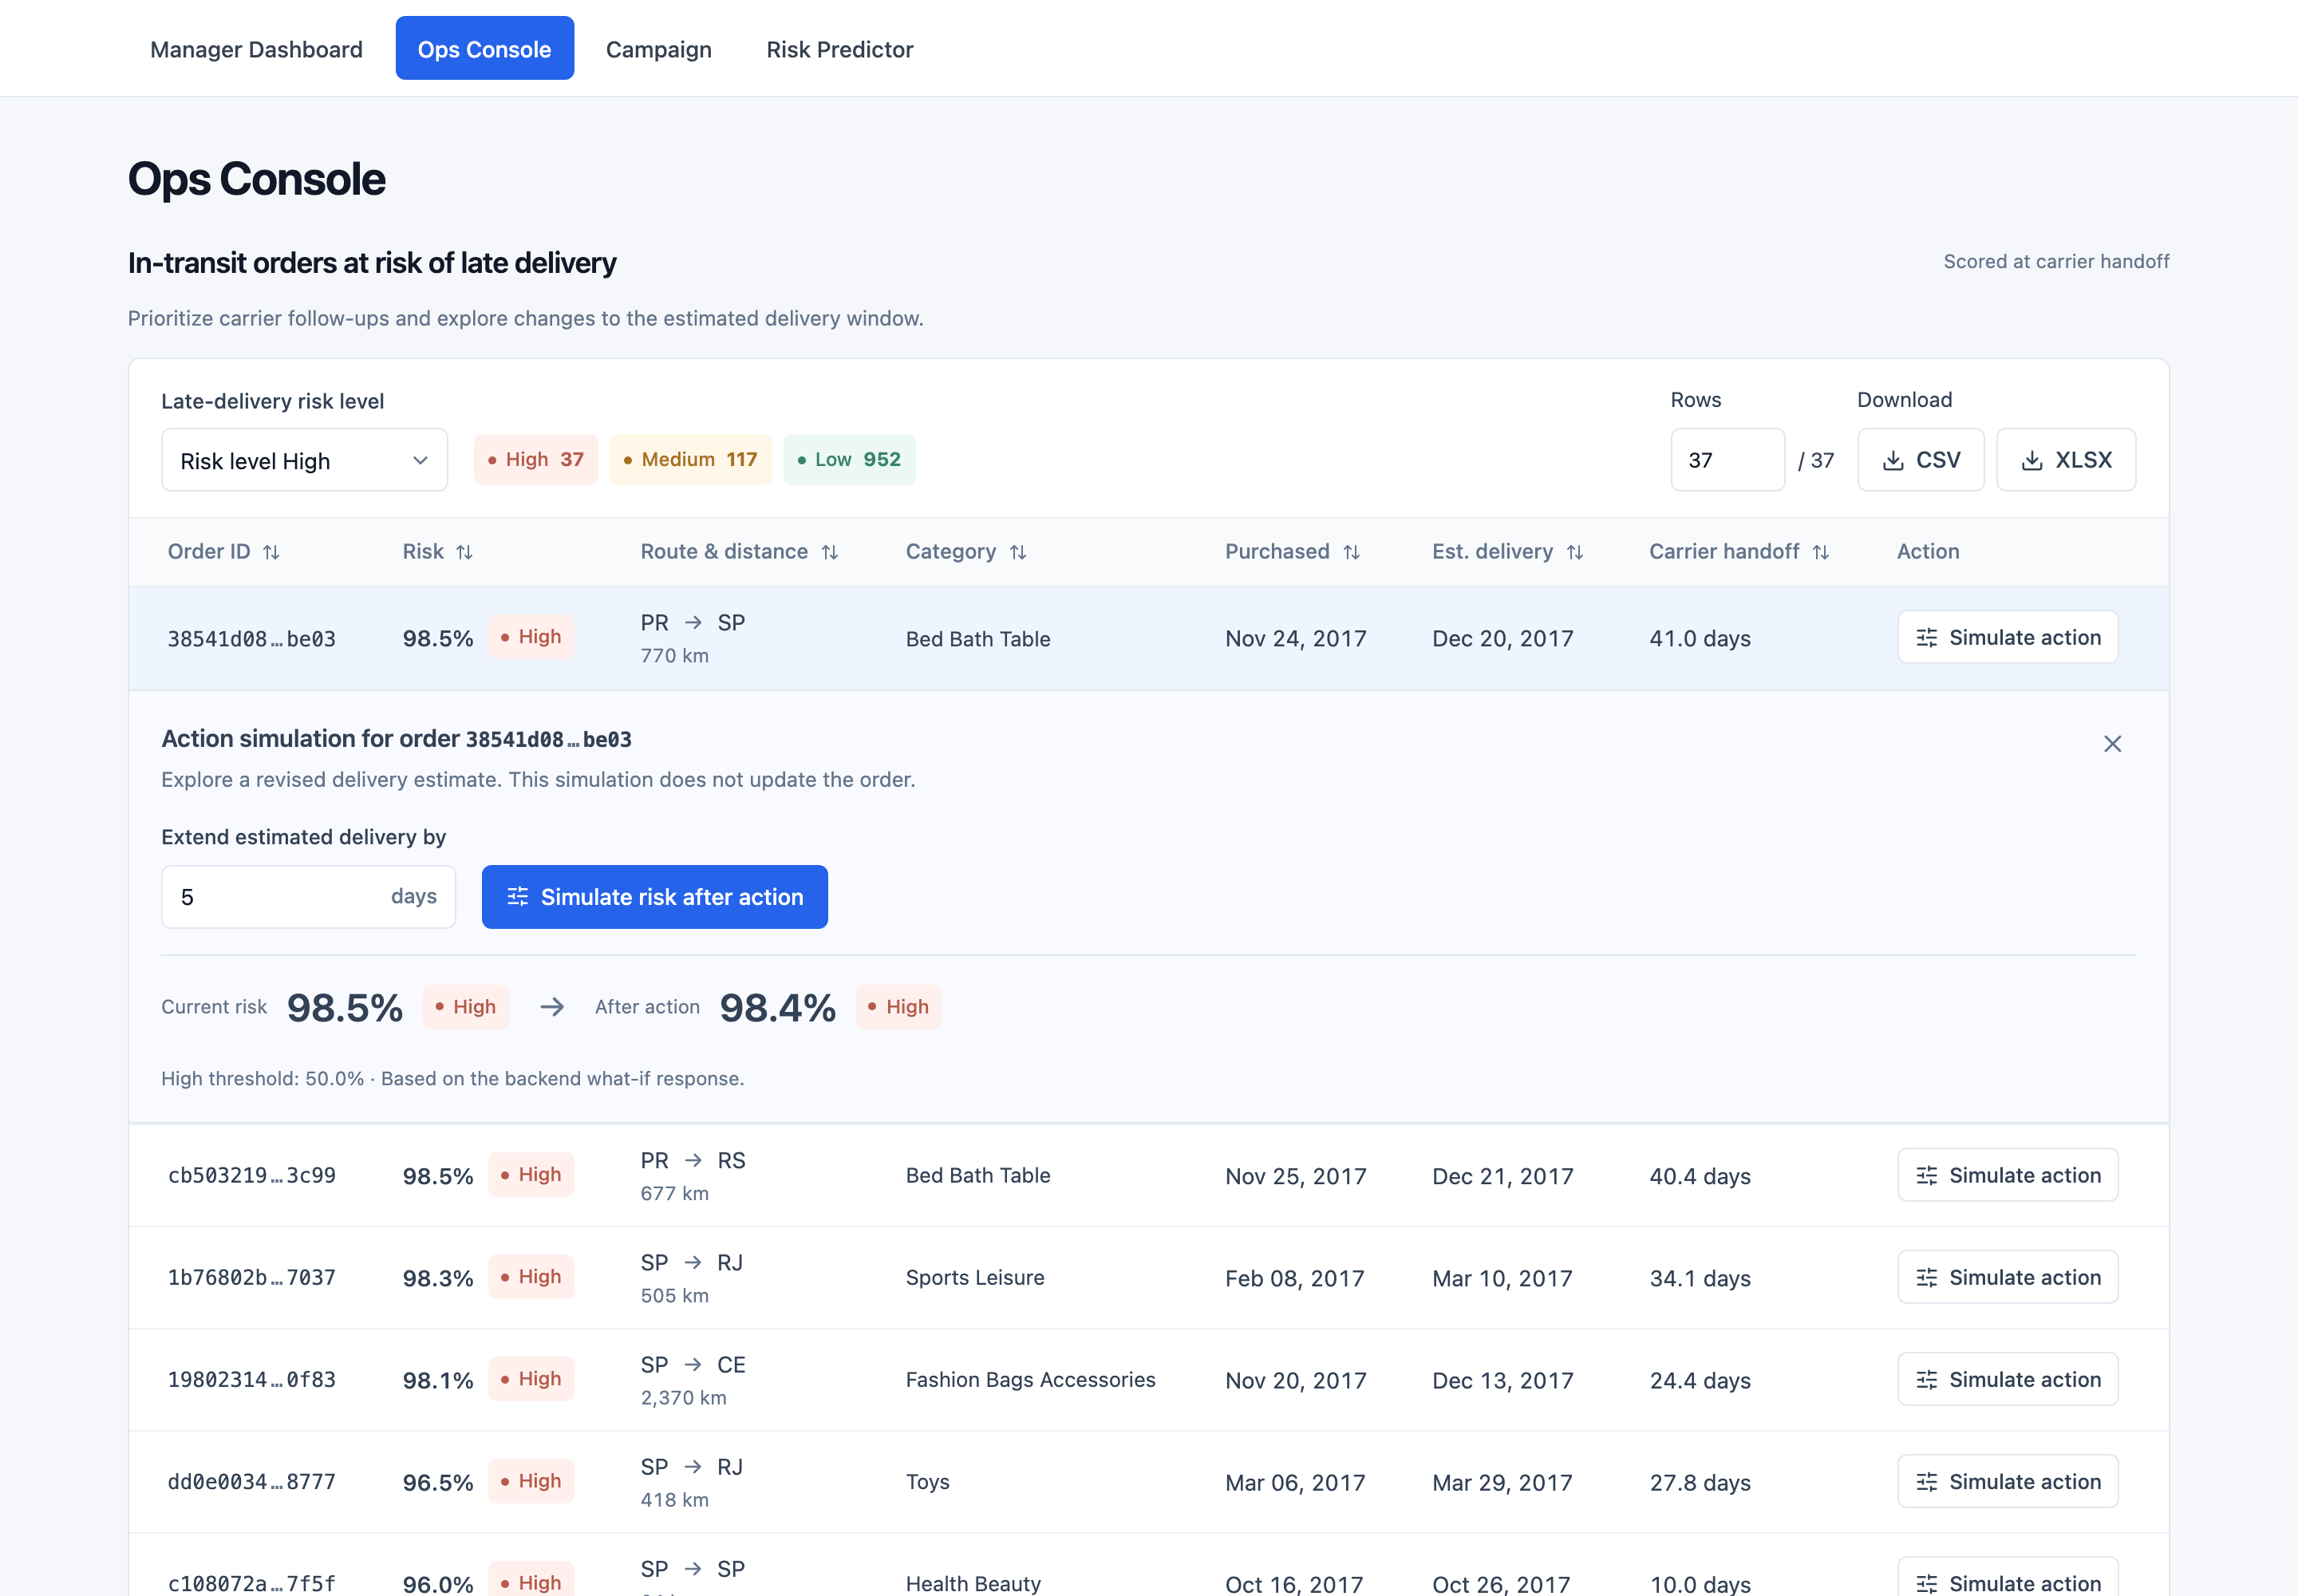
\includegraphics[width=0.75\textwidth]{Picture/ui_ops_late.png}
\caption{Ops Console: danh sách đơn đang vận chuyển có rủi ro giao trễ mức High kèm số đơn theo từng mức, ô chọn số dòng, nút tải CSV/XLSX; khung Action simulation của đơn đầu tiên khi kéo dài ngày hẹn giao 5 ngày (Current risk $\to$ After action)}
\label{fig:ui-ops-late}
\end{figure}

\begin{figure}[H]
\centering
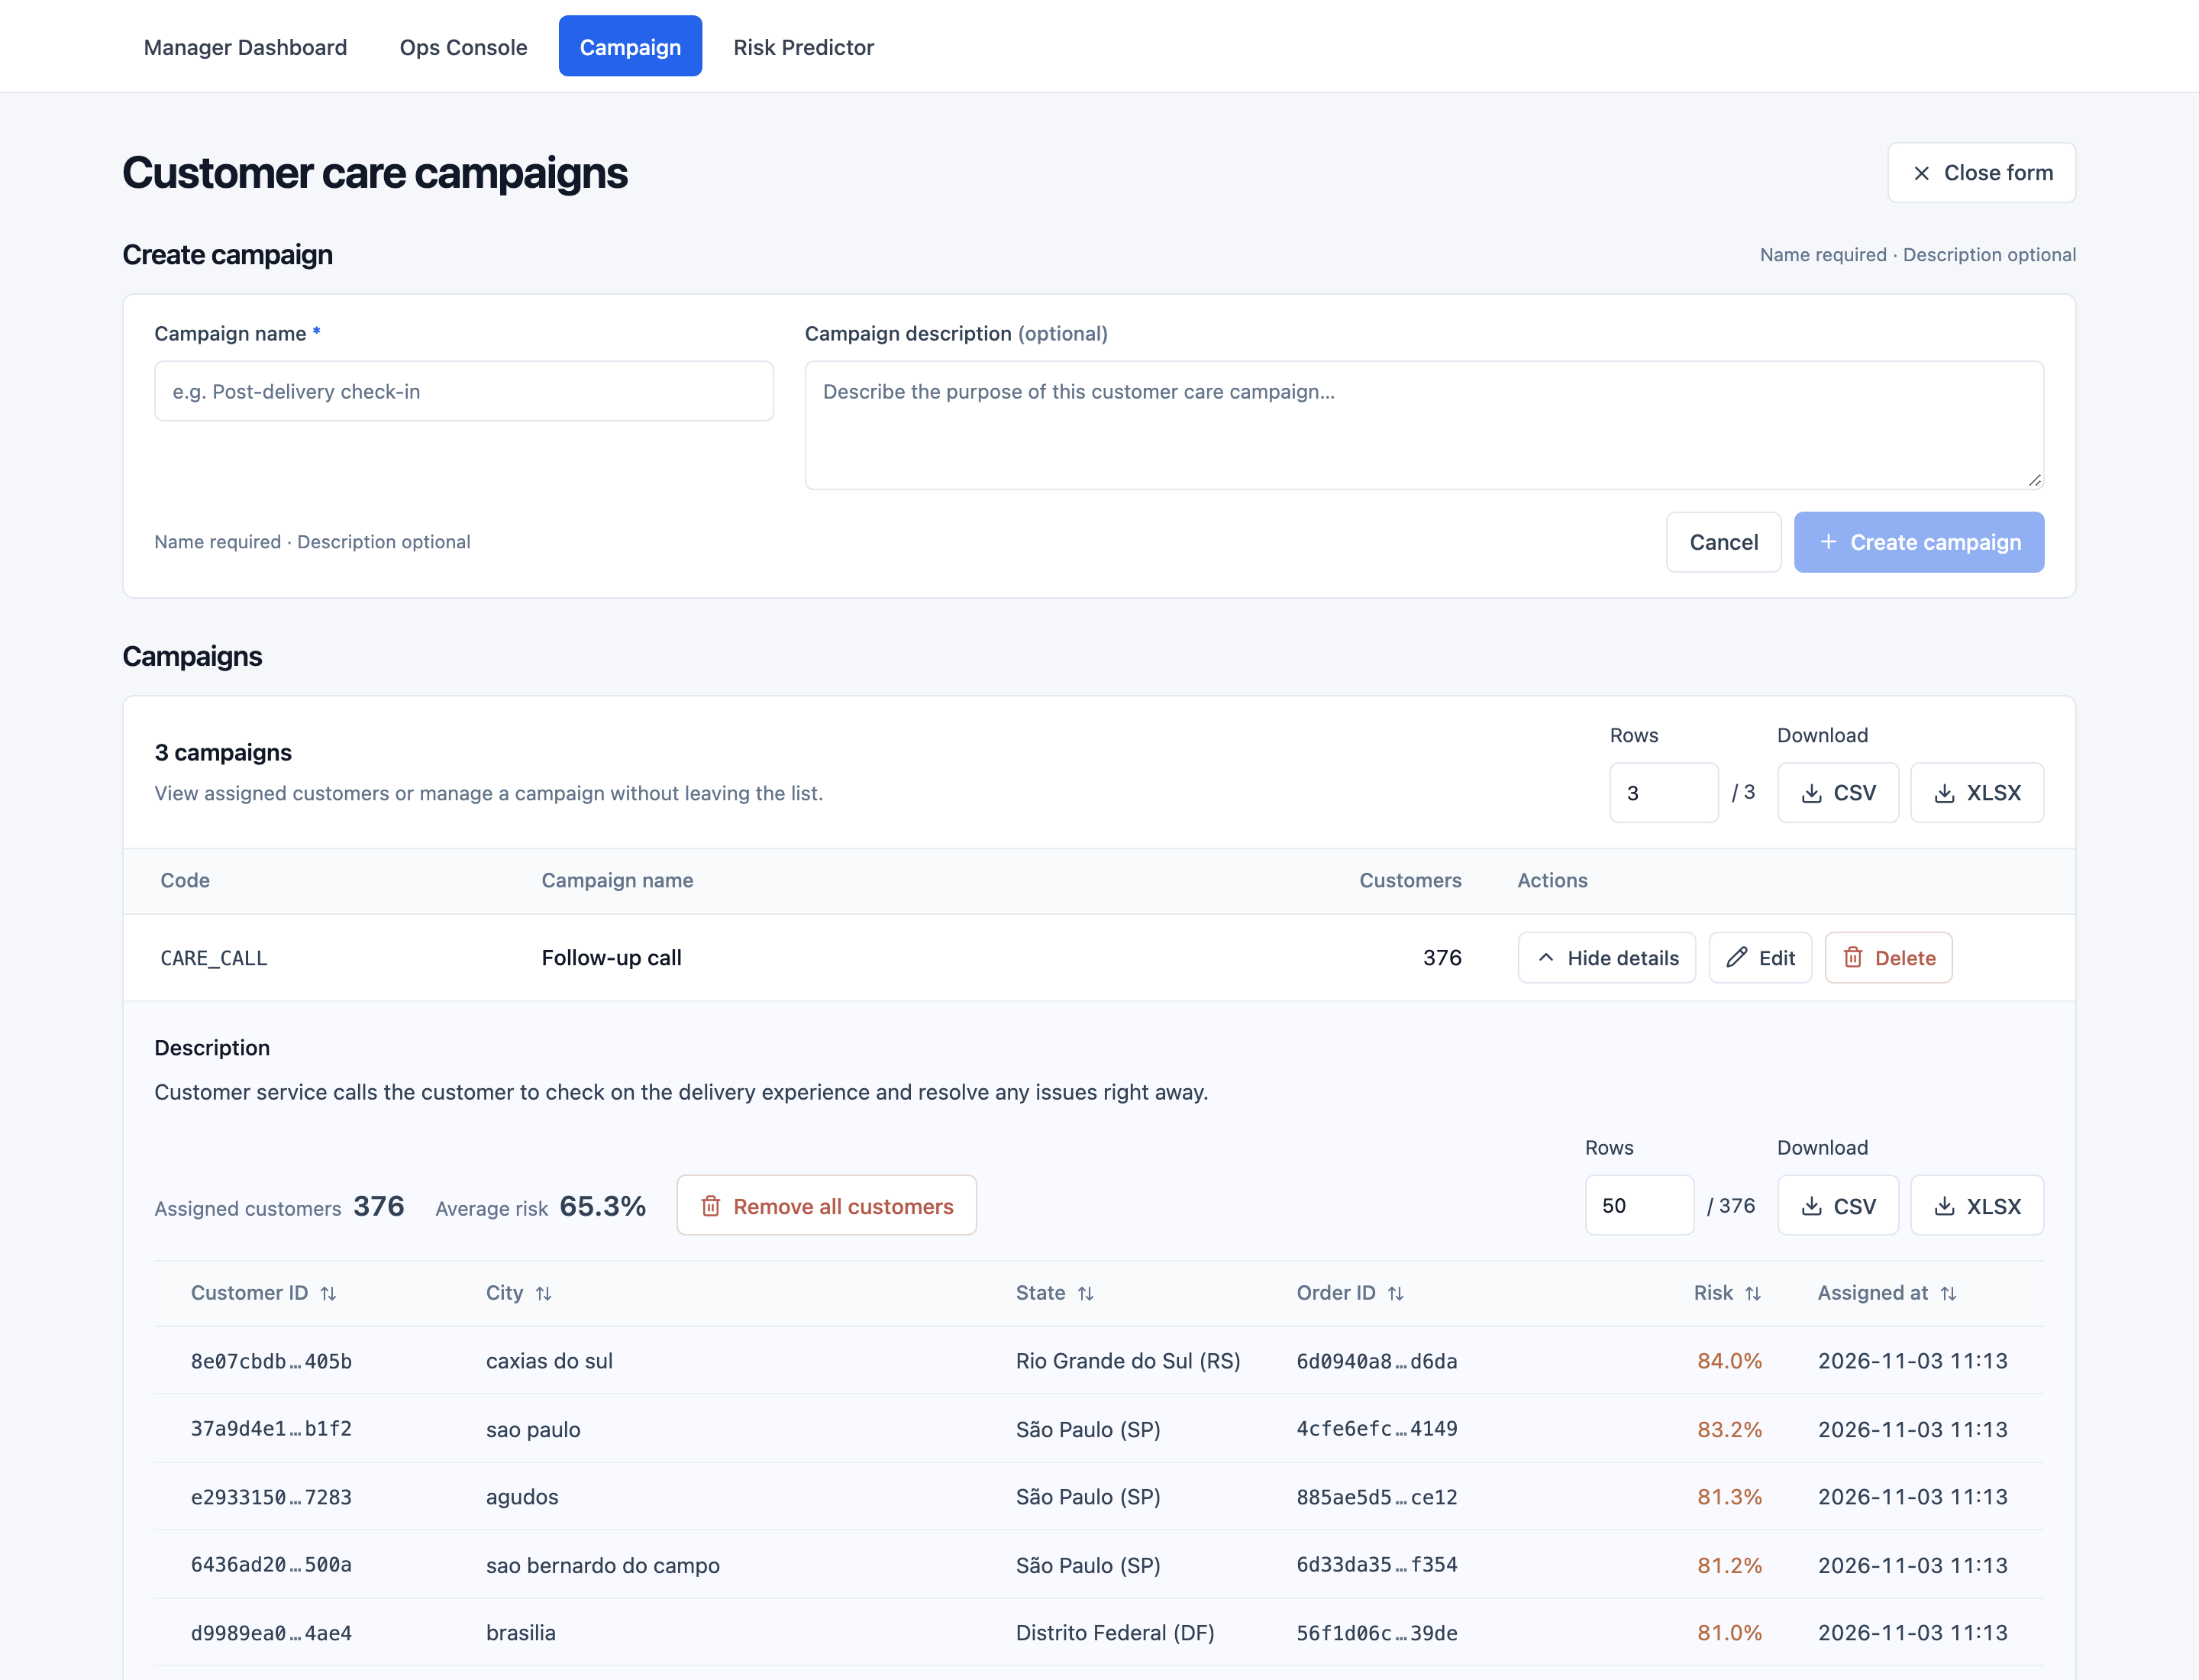
\includegraphics[width=0.75\textwidth]{Picture/ui_campaign.png}
\caption{Màn hình Campaign: danh sách chiến dịch, form thêm mới, phần chi tiết gồm mô tả và khách đã gắn}
\label{fig:ui-campaign}
\end{figure}

\begin{figure}[H]
\centering
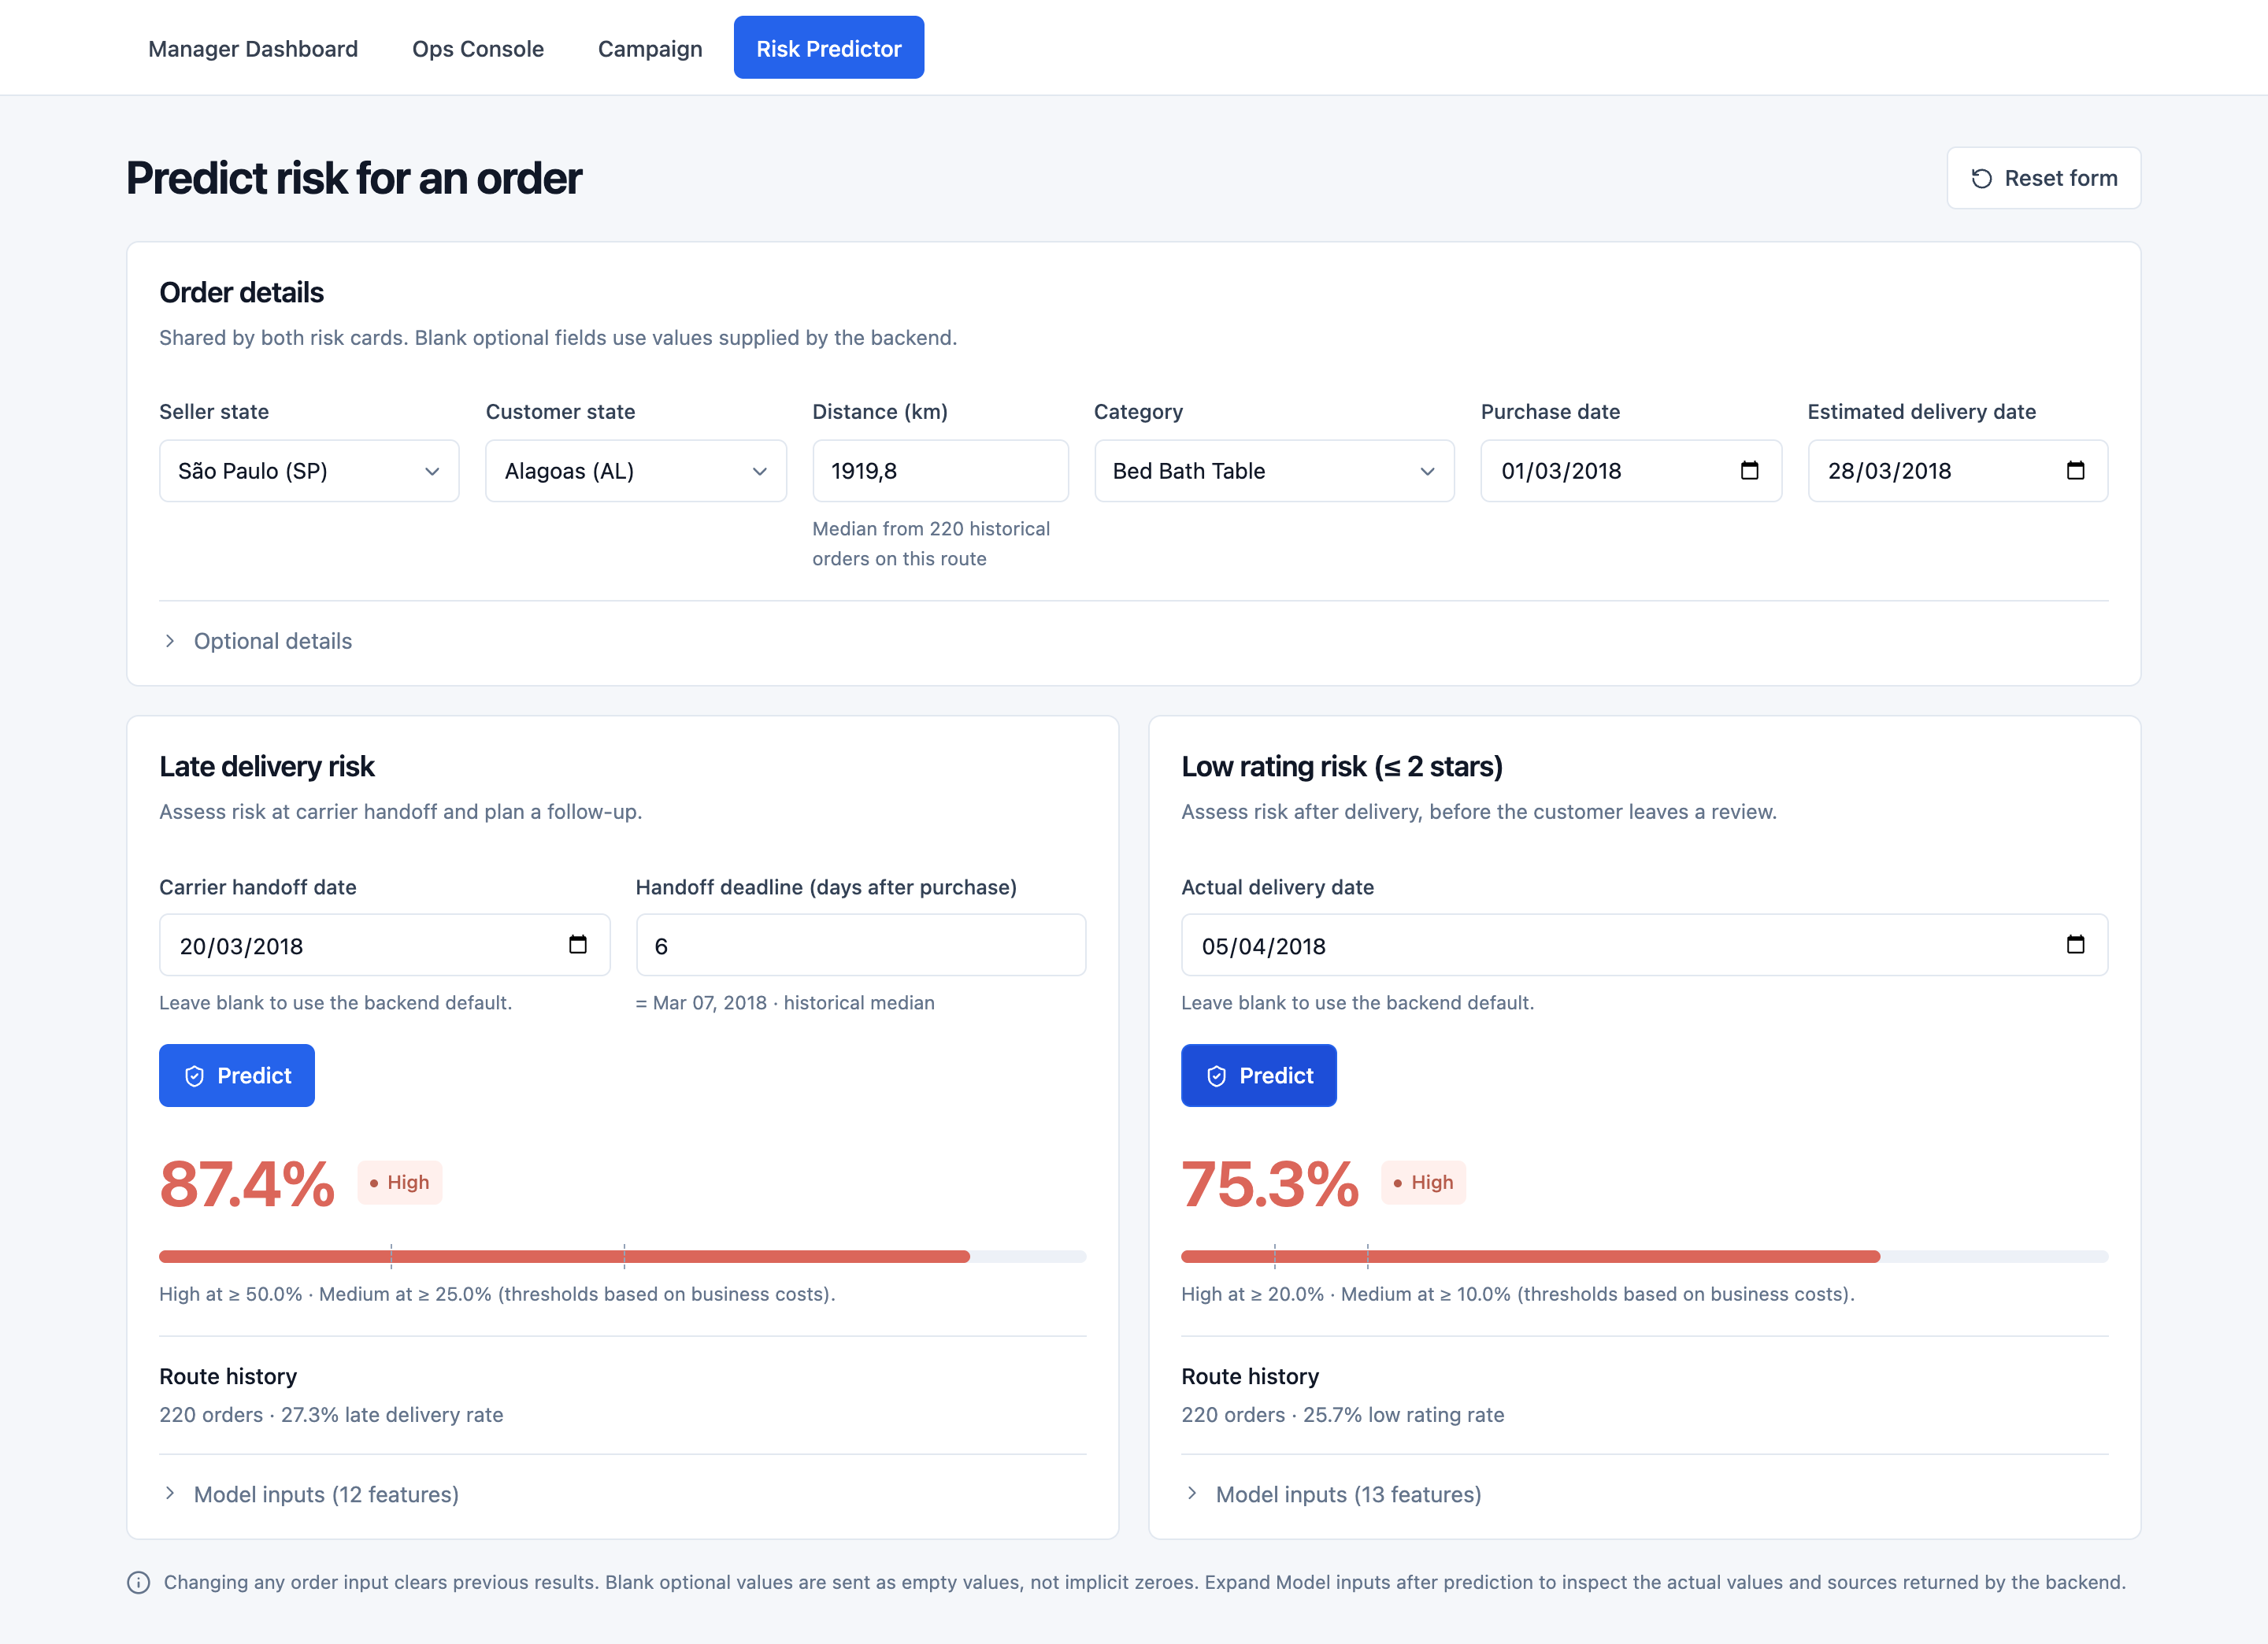
\includegraphics[width=0.75\textwidth]{Picture/ui_predict.png}
\caption{Risk Predictor: đơn giả định tuyến SP $\to$ AL, hẹn giao 27 ngày, người bán bàn giao vào
ngày thứ 19 (rủi ro trễ 87,4\%); nếu giao tới khách trễ 8 ngày thì rủi ro đánh giá thấp 75,3\%}
\label{fig:ui-predict}
\end{figure}


\newpage
% \section{ĐÁNH GIÁ KẾT QUẢ}

\subsection{Kết quả đạt được}
\hspace{1cm}
Toàn bộ pipeline chạy được bằng Airflow trong Docker và bằng script trên máy, kết quả lặp lại
được (chạy ETL lần hai không phát sinh thêm dòng nào). Quy mô dữ liệu đã nạp:
\begin{itemize}
    \item \textbf{Staging}: 99.441 đơn, 112.650 dòng sản phẩm, 103.886 dòng thanh toán, 99.224
          đánh giá, 32.951 sản phẩm, 3.095 người bán, 1.000.163 điểm tọa độ; file cấu hình gồm
          3 chiến dịch chăm sóc mẫu.
    \item \textbf{Dimension}: 96.096 khách hàng với 96.355 phiên bản SCD2 (252 khách đổi địa
          chỉ), 32.951 sản phẩm, 4.310 địa điểm, 3.095 người bán, 5 phương thức thanh toán,
          1.096 ngày; bảng tham chiếu 19.010 zip prefix có tọa độ.
    \item \textbf{Fact}: 112.650 dòng \texttt{FACT\_ORDER\_ITEM}, 98.666 dòng
          \texttt{FACT\_ORDER\_FULFILLMENT} (mọi đơn có sản phẩm; 96.476 đơn đã giao).
    \item \textbf{Chất lượng dữ liệu}: 16/16 kiểm tra đạt.
    \item \textbf{DSS}: 2 mô hình, 38.229 điểm rủi ro theo đơn, chỉ số và feature importance được
          ghi vào kho (trình bày ở Mục~\ref{sec:model-results}); Manager Dashboard và Ops Console
          hiển thị đầy đủ dữ liệu phục vụ vận hành.
\end{itemize}

\subsection{Phân tích mô tả từ kho dữ liệu}
\hspace{1cm}
Truy vấn trên \texttt{FACT\_ORDER\_FULFILLMENT} xác nhận giả thuyết làm nền cho hai mô hình:
giao trễ kéo điểm đánh giá xuống rất mạnh (Bảng~\ref{tab:delay}). Tỷ lệ giao trễ cũng biến
động lớn theo thời gian (03/2018: 19,0\%, 06/2018: 1,2\%) và theo tuyến (SP $\to$ AL: 23,9\%,
SP $\to$ MA: 18,9\%, trong khi trung bình toàn sàn là 6,8\%). Hình~\ref{fig:monthly} cho thấy hai tỷ lệ
biến động cùng chiều: các tháng trễ tăng vọt (11/2017, 02--03/2018) cũng là các tháng tỷ lệ đánh giá
thấp tăng.

\begin{figure}[H]
\centering
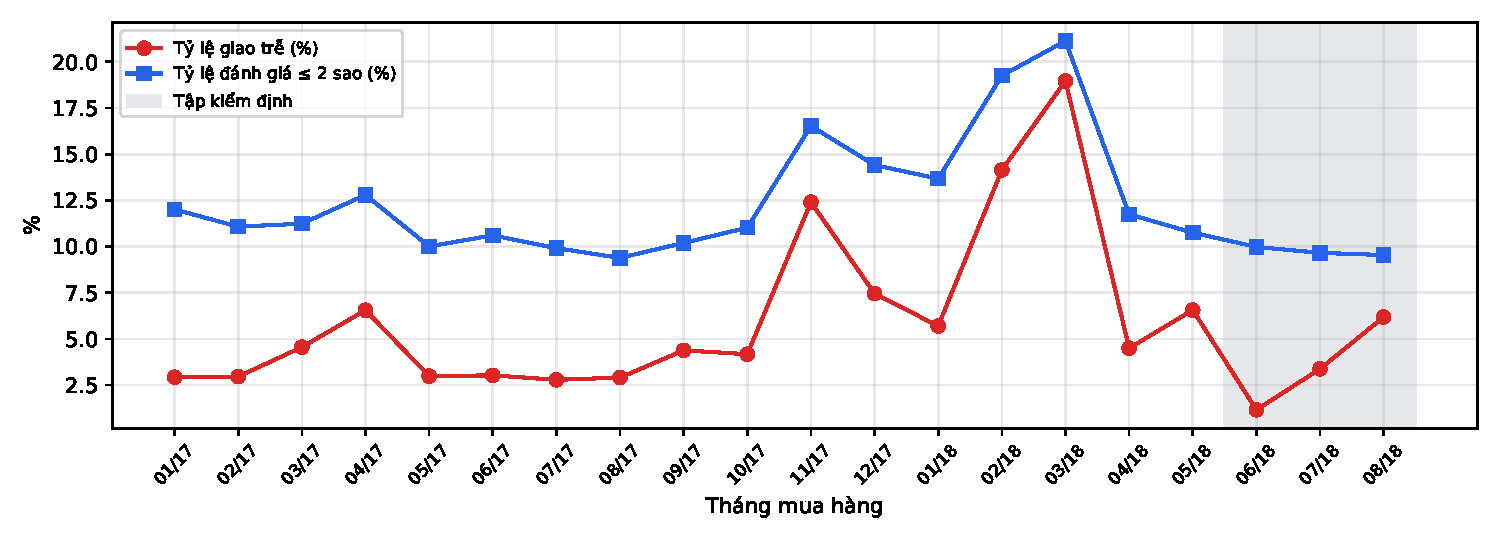
\includegraphics[width=0.95\textwidth]{Picture/monthly_late_review.pdf}
\caption{Tỷ lệ giao trễ và tỷ lệ đánh giá $\leq$ 2 sao theo tháng mua (vùng xám: tập kiểm định)}
\label{fig:monthly}
\end{figure}

\begin{table}[H]
\centering
\caption{Điểm đánh giá theo mức trễ so với ngày hẹn (đơn đã giao, có đánh giá)}
\label{tab:delay}
\begin{tabular}{@{}lrrr@{}}
\toprule
\textbf{Mức trễ} & \textbf{Số đơn} & \textbf{Điểm TB} & \textbf{Tỷ lệ $\leq$ 2 sao} \\
\midrule
Sớm $\geq$ 10 ngày & 61.528 & 4,32 & 8,9\% \\
Sớm 1--9 ngày & 26.640 & 4,23 & 9,9\% \\
Đúng ngày hẹn & 1.280 & 4,04 & 12,3\% \\
Trễ 1--3 ngày & 1.852 & 3,29 & 32,2\% \\
Trễ 4--7 ngày & 1.748 & 2,11 & 67,6\% \\
Trễ $>$ 7 ngày & 2.782 & 1,70 & 79,2\% \\
\bottomrule
\end{tabular}
\end{table}

\subsection{Kết quả hai mô hình DSS}
\label{sec:model-results}
\hspace{1cm}
Bảng~\ref{tab:metrics} tổng hợp chỉ số trên tập kiểm định 06--08/2018 (18.603 đơn cho mô hình
giao trễ, 18.520 đơn cho mô hình đánh giá thấp). PR-AUC cần được so với tỷ lệ nhãn dương (mức
của một mô hình đoán ngẫu nhiên).

\begin{table}[H]
\centering
\caption{Chỉ số đánh giá trên tập kiểm định 06--08/2018}
\label{tab:metrics}
\small\setlength{\tabcolsep}{4pt}
\begin{tabular}{@{}llrrrrrrr@{}}
\toprule
\textbf{Mô hình} & \textbf{Phiên bản} & \textbf{Dương} & \textbf{ROC-AUC} & \textbf{PR-AUC} &
\textbf{Ngưỡng} & \textbf{Prec.} & \textbf{Recall} & \textbf{F1} \\
\midrule
Giao trễ & HGB & 3,6\% & \textbf{0,868} & \textbf{0,519} & 0,5 & \textbf{0,750} & \textbf{0,415} & \textbf{0,534} \\
         & LogReg & 3,6\% & 0,837 & 0,268 & 0,5 & 0,449 & 0,144 & 0,219 \\
Đánh giá thấp & HGB & 9,7\% & \textbf{0,703} & \textbf{0,323} & 0,2 & \textbf{0,415} & \textbf{0,294} & \textbf{0,344} \\
              & LogReg & 9,7\% & 0,689 & 0,285 & 0,2 & 0,414 & 0,275 & 0,331 \\
\bottomrule
\end{tabular}
\end{table}

\begin{itemize}
    \item \textbf{Giao trễ}: PR-AUC 0,519 gấp khoảng 14 lần mức ngẫu nhiên (0,036) và gần gấp
          đôi baseline. Tại ngưỡng 0,5, cứ 4 đơn bị cảnh báo thì 3 đơn trễ thật, và phát hiện
          được 42\% số đơn trễ. Nếu Ops chỉ xử lý 10\% số đơn có điểm cao nhất thì phát hiện được
          63\% số đơn trễ.
    \item \textbf{Đánh giá thấp}: bài toán khó hơn vì điểm đánh giá còn phụ thuộc chất lượng sản
          phẩm, kỳ vọng của khách -- những yếu tố không có trong dữ liệu. PR-AUC 0,323 gấp 3,3 lần
          mức ngẫu nhiên; tại ngưỡng 0,2, 42\% khách được chọn đánh giá thấp thật, gấp 4,3 lần
          nếu chọn ngẫu nhiên.
\end{itemize}

Đường precision--recall (Hình~\ref{fig:pr}) nằm cao hơn hẳn mức ngẫu nhiên ở cả hai mô hình;
với mô hình giao trễ, precision gần 1 ở vùng recall dưới 0,2 (các đơn chắc chắn trễ).

\begin{figure}[H]
\centering
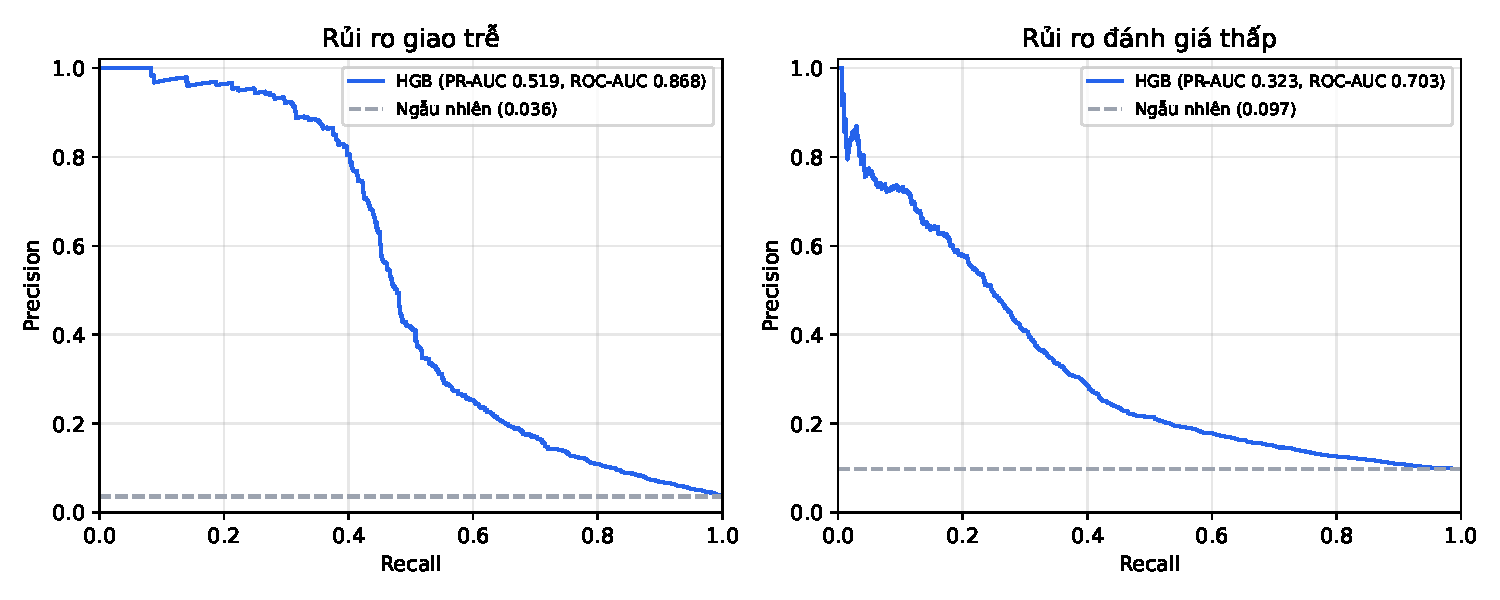
\includegraphics[width=0.95\textwidth]{Picture/pr_curves.pdf}
\caption{Đường precision--recall của mô hình HGB trên tập kiểm định}
\label{fig:pr}
\end{figure}

\textbf{Mức rủi ro có ý nghĩa thực tế} (Bảng~\ref{tab:levels}): tỷ lệ xảy ra thật giảm dần rõ
rệt từ High xuống Low, nên Ops có thể tin vào cách xếp mức để ưu tiên.

\begin{table}[H]
\centering
\caption{Số đơn và tỷ lệ xảy ra thật theo mức rủi ro (tập kiểm định)}
\label{tab:levels}
\begin{tabular}{@{}lrrrr@{}}
\toprule
& \multicolumn{2}{c}{\textbf{Giao trễ}} & \multicolumn{2}{c}{\textbf{Đánh giá thấp}} \\
\textbf{Mức} & \textbf{Số đơn} & \textbf{Trễ thật} & \textbf{Số đơn} & \textbf{$\leq$ 2 sao thật} \\
\midrule
High & 372 & 75,0\% & 1.276 & 41,5\% \\
Medium & 494 & 12,6\% & 2.443 & 12,6\% \\
Low & 17.737 & 1,9\% & 14.801 & 6,5\% \\
\bottomrule
\end{tabular}
\end{table}

\textbf{Đặc trưng quan trọng nhất} (permutation importance, mức giảm PR-AUC, Hình~\ref{fig:importance}):
\begin{itemize}
    \item Giao trễ: \texttt{slack\_days} (0,485) -- số ngày còn lại tới hạn sau khi bàn giao,
          \texttt{handoff\_vs\_\allowbreak limit\_days} (0,074) -- người bán bàn giao muộn so với hạn,
          bang của khách (0,010). Hàm ý: kiểm soát người bán bàn giao đúng hạn là đòn bẩy lớn
          nhất.
    \item Đánh giá thấp: \texttt{delay\_days} (0,127), số sản phẩm trong đơn \texttt{n\_items}
          (0,058), số người bán \texttt{n\_sellers} (0,011). Đơn nhiều sản phẩm/nhiều người
          bán dễ giao thiếu hoặc giao lệch nhau, dẫn tới đánh giá thấp.
\end{itemize}


\begin{figure}[H]
\centering
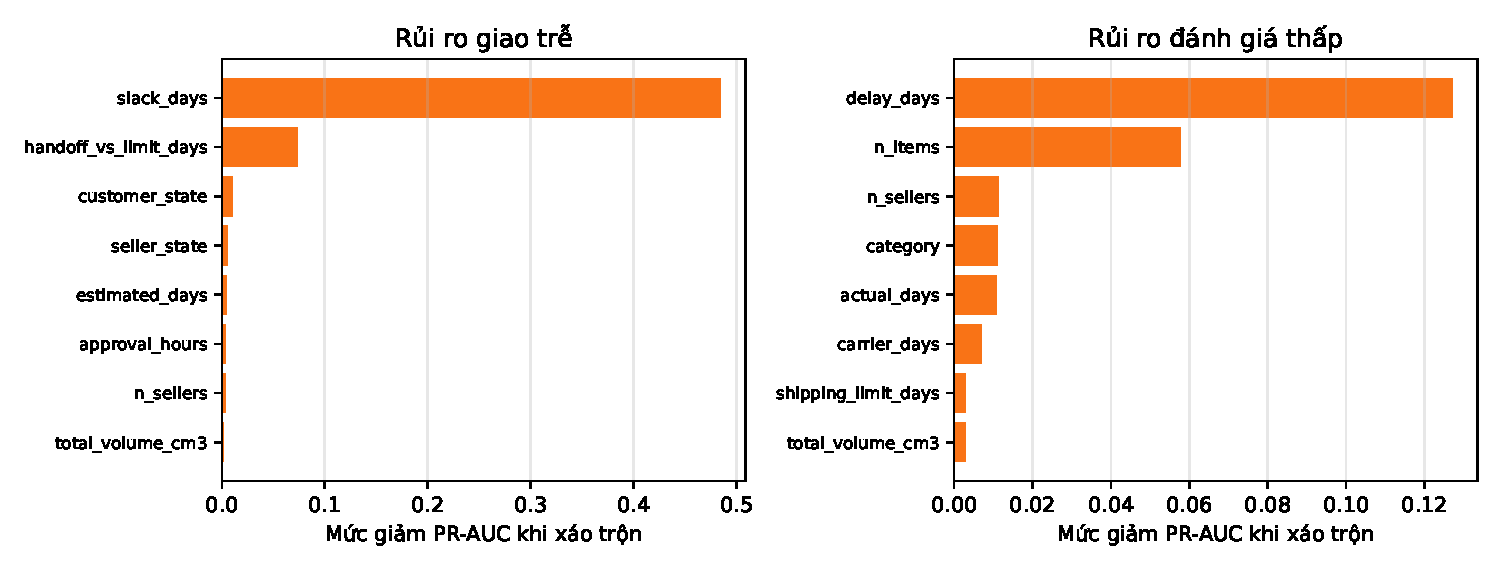
\includegraphics[width=0.95\textwidth]{Picture/feature_importance.pdf}
\caption{Permutation importance (top 8) của hai mô hình HGB}
\label{fig:importance}
\end{figure}

\subsection{Thí nghiệm bổ sung}
\begin{itemize}
    \item \textbf{Chấm điểm sớm hơn (ngay lúc đặt hàng)}: chỉ dùng các đặc trưng có lúc đặt
          hàng thì mô hình giao trễ đạt ROC-AUC 0,693, PR-AUC 0,073 (gần mức ngẫu nhiên); mô hình
          đánh giá thấp đạt ROC-AUC 0,620, PR-AUC 0,186. Điều này giải thích lựa chọn thời điểm
          chấm điểm ở Mục~5.2.
    \item \textbf{Chọn ngưỡng tối đa F1 trên validation}: với mô hình giao trễ, ngưỡng chọn được
          chỉ là 0,07 vì validation (03--05/2018) có tỷ lệ trễ cao bất thường (19\% ở 03/2018),
          áp sang tập kiểm định (3,6\%) cho F1 chỉ 0,207, so với 0,534 khi dùng ngưỡng theo chi
          phí. Với mô hình đánh giá thấp, hai cách cho kết quả gần nhau (0,323 so với 0,344).
          Đây là biểu hiện của \textit{data drift}: tỷ lệ nền thay đổi theo thời gian nên ngưỡng
          nên được đặt từ chi phí nghiệp vụ và được theo dõi định kỳ.
\end{itemize}

\subsection{Hạn chế}
\begin{itemize}
    \item Dataset dừng ở 10/2018 và là dữ liệu lịch sử tĩnh: các đơn ``đang vận chuyển''
          (1.106 đơn) thực chất là đơn bị kẹt trong dữ liệu gốc, nhiều đơn đã quá ngày hẹn.
    \item Không có dữ liệu về hãng vận chuyển, tuyến đường thực tế, thời tiết hay sự kiện (đình
          công, lễ hội) -- nguyên nhân của các đợt trễ tăng vọt -- nên mô hình không dự đoán
          được các cú sốc hệ thống.
    \item Mô hình đánh giá thấp chỉ đạt ROC-AUC 0,70: nội dung đánh giá (văn bản, 58--88\% bị
          trống), chất lượng sản phẩm thực tế không có trong dữ liệu có cấu trúc.
    \item Chi phí $C_{FP}$, $C_{FN}$ là giả định của nhóm, chưa được kiểm chứng bằng dữ liệu
          doanh nghiệp; ngưỡng thay đổi sẽ làm thay đổi precision/recall.
    \item Khoảng cách tính theo tọa độ trung bình của zip prefix và người bán đầu tiên của đơn
          (khoảng 1\% đơn có nhiều người bán).
    \item Công cụ dự đoán cho đơn tự nhập điền các đặc trưng thiếu bằng trung vị nên chỉ phản ánh
          một đơn ``điển hình''; mô hình học tương quan, không phải nhân quả, nên thay đổi các
          đại lượng hiếm gặp trong dữ liệu (như hạn bàn giao rất ngắn) có thể cho kết quả ngược
          trực giác.
    \item Olist là dữ liệu lịch sử nên chức năng gắn khách đang mô phỏng trên các đơn thuộc tập
          kiểm định (đã có review thật); hệ thống cũng chỉ lập danh sách, chưa gửi voucher hay gọi
          khách, nên chưa đo được hiệu quả chăm sóc thật.
\end{itemize}

\subsection{Thiếu sót của đề tài và định hướng mở rộng kho dữ liệu}
\label{sec:dw-gaps}
\hspace{1cm}
Khi đối soát hai bảng fact với các bảng chiều, nhóm nhận thấy nhiều thuộc tính được nạp vào
kho nhưng không có truy vấn nào sử dụng. Để thiết kế gọn và đúng phạm vi đề tài, các thuộc tính
này đã được \textbf{lược bỏ}; bảng chiều chỉ giữ những gì OLAP view, API và mô hình DSS đang
dùng, cùng các khóa tự nhiên cần cho ETL. Đây là một thiếu sót về độ phủ phân tích: kho dữ liệu
hiện trả lời tốt năm câu hỏi nghiệp vụ ở Mục~2.3 nhưng chưa hỗ trợ nhiều góc nhìn ad-hoc.
Bảng~\ref{tab:dropped-attrs} liệt kê các thuộc tính có thể bổ sung lại (dữ liệu nguồn vẫn còn
trong staging) và loại truy vấn ad-hoc mà chúng phục vụ trong tương lai.

\begin{table}[H]
\centering
\caption{Thuộc tính đã lược bỏ và truy vấn ad-hoc có thể phục vụ khi bổ sung lại}
\label{tab:dropped-attrs}
\small
\begin{tabular}{@{}>{\raggedright\arraybackslash}p{2.6cm}>{\raggedright\arraybackslash}p{4.6cm}>{\raggedright\arraybackslash}p{6.8cm}@{}}
\toprule
\textbf{Bảng chiều} & \textbf{Thuộc tính} & \textbf{Truy vấn ad-hoc trong tương lai} \\
\midrule
\texttt{DIM\_DATE} & quý, mùa (Nam bán cầu), cuối tuần, tuần trong năm, tên thứ/tháng &
Phân tích mùa vụ (doanh thu, tỷ lệ trễ theo quý/mùa), so sánh đơn đặt cuối tuần và ngày thường,
báo cáo theo tuần. \\
\texttt{DIM\_PRODUCT} & tên ngành gốc, độ dài tên/mô tả, số ảnh, khối lượng, thể tích &
Chất lượng trang sản phẩm (số ảnh, độ dài mô tả) so với điểm đánh giá; sản phẩm nặng/cồng kềnh
có dễ giao trễ không. \\
\texttt{DIM\_SELLER} & zip, thành phố, vùng & Hiệu suất giao hàng theo vùng hoặc thành phố
của người bán, tuyến vùng $\to$ vùng. \\
\texttt{DIM\_LOCATION} & tên bang, quốc gia & Hiển thị báo cáo bằng tên đầy đủ, mở rộng sang
thị trường ngoài Brazil. \\
\texttt{DIM\_CUSTOMER} & ngày mua đầu tiên & Phân tích cohort, so sánh khách mới và khách quay
lại. \\
\bottomrule
\end{tabular}
\end{table}

Ngược lại, một số \textbf{khóa ngoại} chưa được truy vấn nào dùng nhưng vẫn được \textbf{giữ lại}
vì chúng là khung của star schema và chi phí lưu trữ thấp:
\texttt{customer\_sk}, \texttt{seller\_sk}, \texttt{payment\_type\_sk} trong
\texttt{FACT\_ORDER\_ITEM} (phân tích doanh thu theo khách, người bán, phương thức thanh toán),
và bốn vai trò ngày \texttt{approved\_date\_sk}, \texttt{carrier\_date\_sk},
\texttt{delivered\_date\_sk}, \texttt{estimated\_date\_sk} trong
\texttt{FACT\_ORDER\_FULFILLMENT} (thống kê theo tháng giao hàng hoặc tháng bàn giao thay vì
tháng mua). Định hướng mở rộng:
\begin{itemize}
    \item Bổ sung lại các thuộc tính trong Bảng~\ref{tab:dropped-attrs} khi có câu hỏi nghiệp vụ
          cụ thể, kèm OLAP view và bộ lọc tương ứng trên Manager Dashboard (ví dụ bộ lọc quý,
          mùa).
    \item Xây thêm OLAP view theo các vai trò ngày khác của \texttt{FACT\_ORDER\_FULFILLMENT}
          và theo người bán, khách hàng của \texttt{FACT\_ORDER\_ITEM}.
    \item Duy trì bước đối soát fact -- dimension (khóa NULL, dòng chiều không được tham chiếu,
          thuộc tính không được dùng) như một phần của kiểm tra chất lượng định kỳ; chính bước
          này đã giúp phát hiện lỗi mốc hiệu lực SCD2 theo ngày (Mục~3.2).
\end{itemize}

\subsection{Hướng phát triển}
\begin{itemize}
    \item Chấm điểm lại nhiều lần trong vòng đời đơn (lúc duyệt, lúc bàn giao, mỗi ngày khi đang
          vận chuyển) thay vì một thời điểm cố định.
    \item Thêm đặc trưng lịch sử vận hành (tỷ lệ trễ gần đây theo tuyến, theo người bán) tính
          theo cửa sổ thời gian, kèm cơ chế giám sát drift và tự huấn luyện lại.
    \item Hiệu chỉnh xác suất (\textit{calibration}) và cho phép Ops nhập chi phí trên giao diện
          để tự điều chỉnh ngưỡng.
    \item Đo hiệu quả thật của chiến dịch chăm sóc bằng thử nghiệm A/B (nhóm được tặng voucher và
          nhóm đối chứng) để ước lượng lại $C_{FN}$.
    \item Khai thác nội dung đánh giá (xử lý ngôn ngữ tự nhiên tiếng Bồ Đào Nha) để hiểu nguyên
          nhân đánh giá thấp.
\end{itemize}


\newpage
\section{KẾT LUẬN}

\subsection{Kết luận chung}
\hspace{1cm}
Đồ án đã xây dựng hoàn chỉnh một hệ thống kho dữ liệu và hỗ trợ quyết định cho sàn thương mại
điện tử Olist: kho dữ liệu dạng star schema với hai bảng fact (trong đó
\texttt{FACT\_ORDER\_FULFILLMENT} là \textit{accumulating snapshot} theo vòng đời đơn hàng),
sáu dimension (\texttt{DIM\_CUSTOMER} dùng SCD Type 2 theo địa chỉ), pipeline ETL idempotent
được điều phối bởi Airflow và kiểm tra bằng 16 bài kiểm tra chất lượng dữ liệu, ba OLAP view
phục vụ dashboard. Trên nền kho dữ liệu, hai mô hình DSS dự đoán rủi ro giao trễ (ROC-AUC
0,868, PR-AUC 0,519) và rủi ro nhận đánh giá thấp (ROC-AUC 0,703, PR-AUC 0,323) đều vượt
baseline Logistic Regression, được đánh giá trung thực trên giai đoạn sau giai đoạn huấn luyện,
và được đưa vào quy trình ra quyết định qua ngưỡng theo chi phí, phân tích what-if, chiến
dịch chăm sóc khách hàng trên Ops Console và công cụ dự đoán rủi ro cho một đơn do người dùng tự
nhập (tuyến, ngành hàng, các mốc ngày).

\subsection{Đề xuất hướng phát triển}
\begin{itemize}
    \item Chấm điểm rủi ro nhiều lần trong vòng đời đơn và giám sát drift để tự huấn luyện lại.
    \item Bổ sung dữ liệu vận chuyển (hãng, tuyến, sự kiện) và nội dung đánh giá để cải thiện mô
          hình đánh giá thấp.
    \item Kiểm chứng chi phí và hiệu quả chiến dịch chăm sóc bằng thử nghiệm A/B.
\end{itemize}


\newpage
\section{Tài liệu báo cáo}
\begin{enumerate}
    \item Bộ dữ liệu gốc:\\
    \href{https://www.kaggle.com/datasets/olistbr/brazilian-ecommerce}
    {Kaggle -- Brazilian E-Commerce Public Dataset by Olist}
    \item Github reposity:\\
    \href{https://github.com/MTrang2005/ecommerce-dw-dss}
    {E-commerce DW \& DSS Reposity (Assignment 261)}
    \item Báo cáo (Canva):\\
    \href{https://www.canva.com/design/DAHSK-LCLs0/B5F3qvSOfNbj-x-0ecq62Q/edit}
    {E-commerce DW \& DSS Report}
    
\end{enumerate}

\newpage
\section{Tài liệu tham khảo}
\begin{enumerate}
    \item W. H. Inmon, \textit{Building the Data Warehouse}, 4th ed. Wiley, 2005.
    \item R. Kimball, M. Ross, \textit{The Data Warehouse Toolkit}, 3rd ed. Wiley, 2013.
    \item E. Turban, J. E. Aronson, T.-P. Liang, \textit{Decision Support Systems and
    Intelligent Systems}, 7th ed. Prentice-Hall, 2005.
    \item R. Elmasri, S. B. Navathe, \textit{Fundamentals of Database Systems}, 7th ed.
    Addison-Wesley, 2016.
    \item R. Sharda, D. Delen, E. Turban, \textit{Analytics, Data Science, \& Artificial
    Intelligence: Systems for Decision Support}, 7th ed. Pearson, 2020.
    \item J. Han, M. Kamber, J. Pei, \textit{Data Mining: Concepts and Techniques}, 3rd ed.
    Morgan Kaufmann, 2012.
    \item F. Burstein, C. W. Holsapple, \textit{Handbook on Decision Support Systems}.
    Springer, 2008.
    \item Trần Minh Quang et al., \textit{Cơ sở dữ liệu: khái niệm, phương pháp, và kỹ thuật
    phân tích thiết kế}. NXB ĐHQG-HCM, 2025.
    \item F. Pedregosa et al., ``Scikit-learn: Machine Learning in Python'', \textit{Journal of
    Machine Learning Research}, vol. 12, pp. 2825--2830, 2011.
    \item C. Elkan, ``The Foundations of Cost-Sensitive Learning'', in \textit{Proc. IJCAI},
    2001, pp. 973--978.
\end{enumerate}

\end{document}
